\documentclass[10pt,a4paper]{article}

\usepackage[a4paper,top=1.85cm,bottom=1.85cm,left=1.75cm,right=1.75cm]{geometry}
\usepackage{amsmath,amssymb,mathtools}
\usepackage[T1]{fontenc}
\usepackage{lmodern}
\usepackage{microtype}
\usepackage{graphicx}
\graphicspath{{figs/}}
\usepackage[table]{xcolor}
\usepackage{booktabs}
\usepackage{tabularx}
\usepackage{array}
\usepackage{enumitem}
\usepackage{titlesec}
\usepackage{fancyhdr}
\usepackage{listings}
\usepackage[most]{tcolorbox}
\tcbuselibrary{listings,breakable}
\usepackage{lastpage}
\usepackage{tikz}
\usetikzlibrary{arrows.meta}
\usepackage[hidelinks]{hyperref}

\definecolor{navy}{HTML}{1F3A5F}
\definecolor{teal}{HTML}{0F6E6E}
\definecolor{violet}{HTML}{5B3A8E}
\definecolor{rust}{HTML}{B45309}
\definecolor{lightbg}{HTML}{F7F8FA}
\definecolor{codeblue}{HTML}{0033B3}
\definecolor{codered}{HTML}{A31515}
\definecolor{codegreen}{HTML}{007020}
\definecolor{codegray}{HTML}{7A7A7A}
\colorlet{accent}{navy}

\pagestyle{fancy}
\fancyhf{}
\fancyhead[L]{\small\color{black!65}Numerical Methods --- End-Sem Complete Reference}
\fancyhead[R]{\small\color{black!65}\leftmark}
\fancyfoot[C]{\small\color{black!65}\thepage\ / \pageref{LastPage}}
\setlength{\headheight}{20pt}
\renewcommand{\headrulewidth}{0.3pt}
\renewcommand{\headrule}{\hbox to\headwidth{\color{accent!40}\leaders\hrule height \headrulewidth\hfill}}

\titleformat{\section}
  {\Large\bfseries\color{accent}}
  {\thesection}{0.6em}{}
  [{\vspace{-0.2em}\color{accent}\rule{\linewidth}{0.9pt}}]
\titleformat{\subsection}
  {\large\bfseries\color{accent!90!black}}
  {\thesubsection}{0.5em}{}
\titlespacing*{\section}{0pt}{10pt}{5pt}
\titlespacing*{\subsection}{0pt}{7pt}{3pt}

\setlength{\parindent}{0pt}
\setlength{\parskip}{3.5pt}
\setlength{\abovedisplayskip}{4pt}
\setlength{\belowdisplayskip}{4pt}
\setlist[itemize]{leftmargin=1.2em,itemsep=1pt,topsep=2pt}
\setlist[enumerate]{leftmargin=1.5em,itemsep=1pt,topsep=2pt}
\renewcommand{\arraystretch}{1.18}

\newtcolorbox{keybox}[1][Key result]{
  enhanced, breakable,
  colback=accent!4, colframe=accent!80!black,
  boxrule=0.7pt, arc=1.4mm,
  left=5pt,right=5pt,top=3pt,bottom=3pt,
  title={#1}, fonttitle=\small\bfseries,
  coltitle=white, colbacktitle=accent!80!black
}
\newtcolorbox{derivbox}[1][Derivation]{
  enhanced, breakable,
  colback=black!3, colframe=black!38,
  boxrule=0.5pt, arc=1mm,
  left=5pt,right=5pt,top=3pt,bottom=3pt,
  title={#1}, fonttitle=\small\bfseries,
  coltitle=black, colbacktitle=black!9
}
\newtcolorbox{warnbox}[1][Watch out]{
  enhanced, breakable,
  colback=rust!5, colframe=rust!75!black,
  boxrule=0.6pt, arc=1mm,
  left=5pt,right=5pt,top=3pt,bottom=3pt,
  title={#1}, fonttitle=\small\bfseries,
  coltitle=white, colbacktitle=rust!80!black
}
\newtcolorbox{outbox}[1][Program Output]{
  enhanced, breakable,
  colback=black!2, colframe=black!45,
  boxrule=0.5pt, arc=1mm,
  left=5pt,right=5pt,top=3pt,bottom=3pt,
  title={#1}, fonttitle=\small\bfseries,
  coltitle=white, colbacktitle=black!65
}
\newtcolorbox{overviewbox}[2][]{
  enhanced, colback=#1!5, colframe=#1!80!black,
  boxrule=0.6pt, arc=1.2mm,
  left=5pt,right=5pt,top=3pt,bottom=3pt,
  title={#2}, fonttitle=\small\bfseries,
  coltitle=white, colbacktitle=#1!80!black
}

\newtcblisting{jupytercode}[1][Python Reference Code]{
  colback=lightbg,
  colframe=accent!45,
  listing only,
  breakable,
  title={\small\bfseries #1},
  coltitle=white,
  colbacktitle=accent!75!black,
  left=12pt,
  right=4pt,
  top=2pt,
  bottom=2pt,
  boxrule=0.5pt,
  arc=1.2mm,
  listing options={
    language=Python,
    basicstyle=\ttfamily\footnotesize\color{black},
    keywordstyle=\color{codeblue}\bfseries,
    commentstyle=\color{codegreen}\itshape,
    stringstyle=\color{codered},
    numberstyle=\tiny\color{codegray},
    numbers=left,
    stepnumber=1,
    numbersep=6pt,
    showstringspaces=false,
    breaklines=true,
    tabsize=4
  }
}

\newcommand{\dd}{\mathrm{d}}
\newcommand{\x}{\mathbf{x}}
\newcommand{\R}{\mathbb{R}}
\newcommand{\avg}[1]{\left\langle #1 \right\rangle}

\begin{document}

%============================================================
% TITLE + COURSE MAP + TOC
%============================================================
\begin{center}
{\color{navy}\rule{\linewidth}{2pt}}\\[0.5em]
{\Huge\bfseries Numerical Methods}\\[10pt]
{\LARGE End-Semester Complete Notes, Full Code \& Outputs}\\[6pt]
{\large Linear ODEs \quad$\cdot$\quad Nonlinear ODEs \quad$\cdot$\quad Linear PDEs \quad$\cdot$\quad Stochastic Systems \quad$\cdot$\quad Manual Linear Solve}\\[3pt]
{\small Phy 324 --- Theory, Derivations, Problem Set Solutions, Full Runnable Scripts \& Rendered Output Plots}\\[0.4em]
{\color{navy}\rule{\linewidth}{2pt}}
\end{center}

\vspace{0.2em}
{\color{navy}\Large\bfseries The Whole Syllabus on One Page}

\vspace{0.25em}
\noindent
\begin{minipage}[t]{0.487\textwidth}
\begin{overviewbox}[navy]{1. Linear ODEs}
\begin{itemize}
\item Explicit, Improved (Heun) \& Implicit Euler
\item Stability: $\Delta t \le 2/\lambda$ (Explicit), unconditional (Implicit)
\item Damped/Driven SHM $\to$ 1st-order vector system
\item Euler-Cromer vs Simple Euler energy blowup; RK4 ($O(h^4)$)
\item 2D linear $\dot{\mathbf{x}}=J\mathbf{x}$: eigenvalues, $\tau$-$\Delta$ plane
\end{itemize}
\end{overviewbox}
\vspace{0.2em}
\begin{overviewbox}[teal]{2. Nonlinear ODEs}
\begin{itemize}
\item Fixed points $f(x^*)=0$, linear test $f'(x^*)<0$
\item 1D bifurcations: Saddle-Node, Transcritical, Pitchfork
\item Rotating hoop ($\omega_c^2=g/r$) \& overdamped reduction
\item 2D nonlinear phase plane: nullclines \& Jacobian $J$
\item Multivariable Newton-Raphson ($J\Delta x = -F$)
\end{itemize}
\end{overviewbox}
\end{minipage}\hfill
\begin{minipage}[t]{0.487\textwidth}
\begin{overviewbox}[violet]{3. Linear PDEs}
\begin{itemize}
\item Symmetries, Dirichlet / Neumann (no-flux) / Periodic BCs
\item 1D Diffusion: FTCS ($C\le 1/2$), BTCS (unconditional)
\item 2D Diffusion ($C\le 1/4$), $d$-D ($1/2d$), Heterogeneous $D(x)$
\item Fourier mode decay: $\tau_k = 1/(Dk^2) = \lambda^2/(4\pi^2 D)$
\item Advection Upwind ($K\le 1$) \& 2nd-Order Wave Leap-Frog ($K=1$)
\end{itemize}
\end{overviewbox}
\vspace{0.2em}
\begin{overviewbox}[rust]{4. Stochastic Systems \& Manual Linear Solve}
\begin{itemize}
\item 1D/2D Random walks: $\avg{x_n^2}=n$, $\avg{R_n^2}=2n$
\item Biased walk: $\avg{x_n}=n(p-q)$, $\text{Var}(x_n)=4npq$
\item Langevin ($m\dot v=-\gamma v+\xi$), Einstein $D=k_B T/\gamma$
\item Euler-Maruyama ($\sqrt{2D\Delta t}\,\eta_n$) \& Fokker-Planck
\item Manual $A\mathbf{x}=\mathbf{b}$ solve (Gaussian elimination + pivoting)
\end{itemize}
\end{overviewbox}
\end{minipage}

\vspace{0.3em}
\begin{keybox}[Notation and the Core Idea]
\[
t_n = t_0 + n\Delta t,\qquad y_n \approx y(t_n),\qquad x_i = i\Delta x,\qquad L = N\Delta x.
\]
Replace derivatives with finite differences to turn differential equations into algebraic updates. Every exam question asks: \textbf{(1) How accurate is it?} (order/truncation error) and \textbf{(2) Does error blow up?} (stability condition). Every script in this PDF is \textbf{complete and runnable as printed}, paired directly with its exact rendered output figure.
\end{keybox}

\vspace{0.2em}
\tableofcontents

%============================================================
\clearpage
\colorlet{accent}{navy}
\section{Linear Ordinary Differential Equations}
{\sloppy\small\emph{Notebooks covered: \texttt{01\_First\_Order\_ODEs\_and\_Euler\_Methods.ipynb}, \texttt{02\_Second\_Order\_ODEs\_SHM\_and\_RK4.ipynb}, \texttt{03\_2D\_Linear\_Autonomous\_Systems.ipynb}, \texttt{04\_Linear\_ODE\_Problem\_Set\_Solutions.ipynb}. Sources: \texttt{lec9--11.pdf}, \texttt{Problem Set II Q1, Q3}, \texttt{problem\_set\_III Q1}, \texttt{Nuclear-decay.ipynb}, \texttt{SHM\_rk4.ipynb}, \texttt{Simple Harmonic Ocilator.ipynb}.}\par}

\subsection{First-Order Linear ODEs \& Decay Model}
A first-order linear ODE has the form $y'+p(t)y=q(t)$ with integrating factor $\mu(t)=e^{\int p(t)\dd t}$, giving $y(t)=\frac{1}{\mu(t)}(C+\int \mu(t)q(t)\dd t)$. The standard model and stability test equation is radioactive decay:
\[
\boxed{\;\frac{\dd N}{\dd t}=-\lambda N \quad\Longrightarrow\quad N(t)=N_0e^{-\lambda t},\qquad \tau=\frac{1}{\lambda},\qquad t_{1/2}=\frac{\ln 2}{\lambda}\;}
\]
Here $\tau = 1/\lambda$ is the characteristic decay timescale (time for $N$ to drop by a factor of $e$).

\subsection{Explicit, Improved, and Implicit Euler Methods}

\begin{derivbox}[Euler Error \& Stability on $y' = -\lambda y$ ($\lambda > 0$, step $\Delta t = h$)]
Taylor expand $y(t+h)=y(t)+h y'(t)+\frac{h^2}{2}y''(c)$. Dropping $\frac{h^2}{2}y''(c)$ gives:
\begin{itemize}
\item \textbf{Simple (Explicit) Euler:} $y_{n+1} = y_n + h f(t_n, y_n)$. Local error $O(h^2)$; over $N=T/h$ steps, global error $= N\cdot O(h^2) = O(h)$ (1st order).
On $y'=-\lambda y$: $y_{n+1} = (1 - \lambda h)y_n \implies y_n = (1-\lambda h)^n y_0$. Boundedness requires $|1-\lambda h| \le 1 \implies \mathbf{h \le \frac{2}{\lambda}}$.
\item \textbf{Improved Euler (Heun):} $y_p = y_n + h f(t_n,y_n)$, then $y_{n+1} = y_n + \frac{h}{2}[f(t_n,y_n)+f(t_{n+1},y_p)]$. Local error $O(h^3)$, global error $O(h^2)$ (2nd order). For $y'=-\lambda y$: $y_{n+1} = (1 - \lambda h + \frac{1}{2}(\lambda h)^2)y_n$, stable for $0 \le \lambda h \le 2$.
\item \textbf{Implicit (Backward) Euler (Problem Set III Q1):} Evaluates slope at future step $y_{n+1} = y_n + h f(t_{n+1}, y_{n+1})$.
On $y'=-\lambda y$: $y_{n+1} = y_n - \lambda h y_{n+1} \implies \mathbf{y_{n+1} = \frac{y_n}{1+\lambda h}}$. Since $|\frac{1}{1+\lambda h}| < 1$ for all $h > 0$, it is \textbf{unconditionally stable}.
\end{itemize}
\end{derivbox}

\begin{keybox}[Explicit vs Implicit Stability Summary]
\begin{itemize}
\item $h < 1/\lambda$: smooth monotone decay (positivity-preserving).
\item $1/\lambda < h < 2/\lambda$: decays, but flips sign every step (unphysical oscillations).
\item $h > 2/\lambda$: Explicit Euler blows up; Implicit Euler remains stable for \textbf{all} $h > 0$.
\end{itemize}
\end{keybox}

\begin{jupytercode}[1st-Order Decay: Simple, Improved \& Implicit Euler (Stable dt = 0.5)]
import numpy as np
import matplotlib.pyplot as plt

# Compare Simple Euler, Improved Euler, and Implicit Euler (stable step size)
lam = 0.5
N0 = 100.0
dt = 0.5      # 1/lam = 2.0, so dt = 0.5 is well inside stability limit
t = np.arange(0, 10 + dt, dt)
n = len(t)

N_exact = N0 * np.exp(-lam * t)
N_euler = np.zeros(n)
N_imp = np.zeros(n)
N_implicit = np.zeros(n)

N_euler[0] = N0
N_imp[0] = N0
N_implicit[0] = N0

for i in range(n - 1):
    N_euler[i + 1] = N_euler[i] * (1 - lam * dt)
    N_imp[i + 1] = N_imp[i] * (1 - lam * dt + 0.5 * (lam * dt)**2)
    N_implicit[i + 1] = N_implicit[i] / (1 + lam * dt)

plt.figure(figsize=(7, 4))
plt.plot(t, N_exact, 'k-', label='Exact')
plt.plot(t, N_euler, 'o--', label='Simple Euler')
plt.plot(t, N_imp, 's-', label='Improved Euler')
plt.plot(t, N_implicit, '^-', label='Implicit Euler')
plt.xlabel('t')
plt.ylabel('N(t)')
plt.title(f'Nuclear Decay Methods (dt = {dt}, 1/lam = {1/lam})')
plt.legend()
plt.grid(True)
plt.show()
\end{jupytercode}
\begin{center}
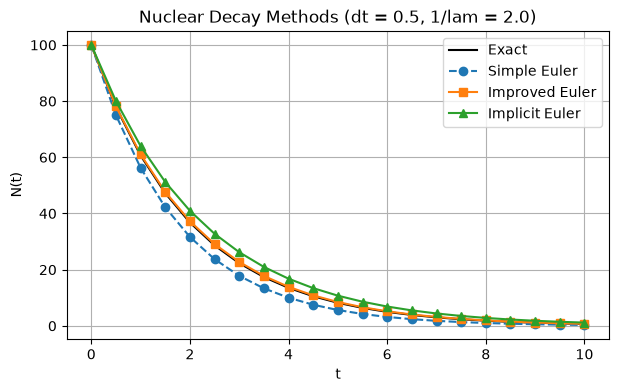
\includegraphics[width=0.72\linewidth]{Linear_Ordinary_Differential_Equations__01_First_Order_ODEs_and_Euler_Methods__c1_o0.png}
\end{center}

\begin{jupytercode}[Stability Check: Explicit Blowup vs Implicit Stability (dt = 4.2 > 2/lam)]
import numpy as np
import matplotlib.pyplot as plt

lam = 0.5
N0 = 100.0
dt_big = 4.2   # Instability demonstration when dt > 2 / lam (here 2 / lam = 4.0)
t_big = np.arange(0, 25 + dt_big, dt_big)
n_big = len(t_big)

N_exp_big = np.zeros(n_big)
N_imp_big = np.zeros(n_big)
N_exp_big[0] = N0
N_imp_big[0] = N0

for i in range(n_big - 1):
    N_exp_big[i + 1] = N_exp_big[i] * (1 - lam * dt_big)
    N_imp_big[i + 1] = N_imp_big[i] / (1 + lam * dt_big)

plt.figure(figsize=(7, 4))
plt.plot(t_big, N_exp_big, 'r-o', label='Explicit Euler (Blows up!)')
plt.plot(t_big, N_imp_big, 'g-s', label='Implicit Euler (Stable)')
plt.xlabel('t')
plt.ylabel('N(t)')
plt.title(f'Stability Check at dt = {dt_big} > 2/lam = 4.0')
plt.legend()
plt.grid(True)
plt.show()
\end{jupytercode}
\begin{center}
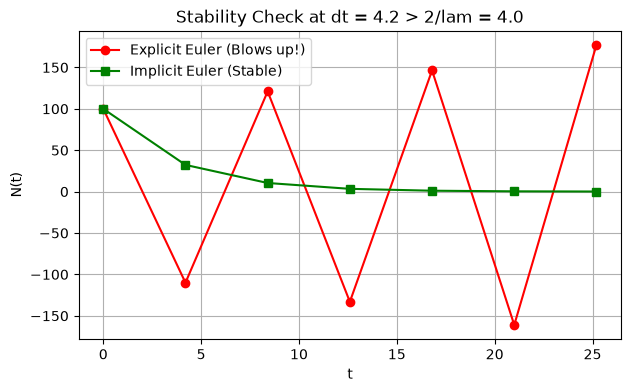
\includegraphics[width=0.72\linewidth]{Linear_Ordinary_Differential_Equations__01_First_Order_ODEs_and_Euler_Methods__c2_o0.png}
\end{center}

\begin{jupytercode}[Exact Class Code: Nuclear Decay (Notes/Nuclear-decay.ipynb)]
import numpy as np
import matplotlib.pyplot as plt

def decay(init_particles, lamb, time):
    return init_particles * np.exp(-lamb * time)

def simple_euler(N0, lamb, dt, n):
    N = np.zeros(n)
    N[0] = N0
    for i in range(n - 1):
        N[i + 1] = N[i] * (1 - lamb * dt)
    return N

def improved_euler(N0, lamb, dt, n):
    N = np.zeros(n)
    N[0] = N0
    for i in range(n - 1):
        N[i + 1] = N[i] * (1 - lamb * dt * (1 - lamb * dt * 0.5))
    return N

dt_c = 1.0
t_c = np.arange(0, 10 + dt_c, dt_c)
plt.figure(figsize=(7, 4))
plt.plot(t_c, decay(1000, 0.2, t_c), 'k-', label='Analytical')
plt.plot(t_c, simple_euler(1000, 0.2, dt_c, len(t_c)), 'o--', label='Simple Euler')
plt.plot(t_c, improved_euler(1000, 0.2, dt_c, len(t_c)), 's-', label='Improved Euler')
plt.xlabel('Time')
plt.ylabel('Particles')
plt.title('Class Code Output (n/Nuclear-decay.ipynb)')
plt.legend()
plt.grid(True)
plt.show()
\end{jupytercode}
\begin{center}
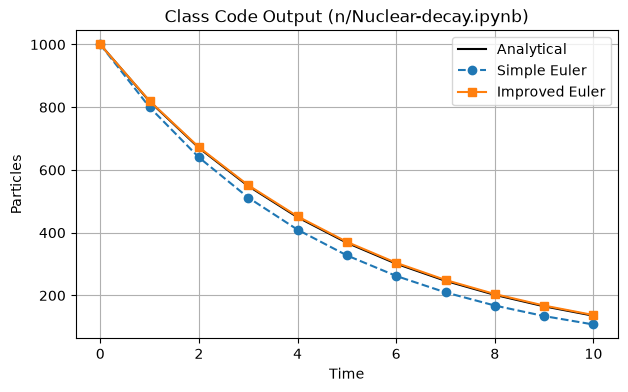
\includegraphics[width=0.72\linewidth]{Linear_Ordinary_Differential_Equations__01_First_Order_ODEs_and_Euler_Methods__c4_o0.png}
\end{center}

\begin{jupytercode}[Exam Variation: General 1st-Order ODE dy/dt = f(t, y) via Improved Euler]
import numpy as np
import matplotlib.pyplot as plt

# General Improved Euler example: dy/dt = -2*y + sin(t), y(0) = 1
def f_general(t_val, y_val):
    return -2.0 * y_val + np.sin(t_val)

dt_g = 0.05
t_g = np.arange(0, 5 + dt_g, dt_g)
y_g = np.zeros(len(t_g))
y_g[0] = 1.0

for i in range(len(t_g) - 1):
    y_p = y_g[i] + dt_g * f_general(t_g[i], y_g[i])
    y_g[i + 1] = y_g[i] + 0.5 * dt_g * (f_general(t_g[i], y_g[i]) + f_general(t_g[i] + dt_g, y_p))

plt.figure(figsize=(6, 3.5))
plt.plot(t_g, y_g, 'b-', label='General Improved Euler')
plt.xlabel('t'); plt.ylabel('y(t)')
plt.title('General 1st-Order ODE: dy/dt = -2y + sin(t)')
plt.legend(); plt.grid(True); plt.show()
\end{jupytercode}
\begin{center}
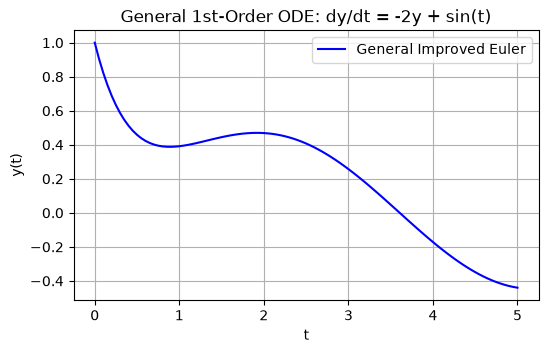
\includegraphics[width=0.68\linewidth]{Linear_Ordinary_Differential_Equations__01_First_Order_ODEs_and_Euler_Methods__c6_o0.png}
\end{center}

\begin{jupytercode}[Problem Set III Q1: Explicit vs Implicit Euler (dt = 1.1 > 2/lam = 1.0)]
import numpy as np
import matplotlib.pyplot as plt

lam = 2.0   # stability limit for explicit Euler is dt < 2/lam = 1.0
y0 = 1.0
dt = 1.1    # larger than 2/lam -> explicit blows up, implicit stays stable

t = np.arange(0, 10, dt)
n = len(t)
y_exp = np.zeros(n)
y_imp = np.zeros(n)
y_exp[0] = y0
y_imp[0] = y0

for i in range(n - 1):
    y_exp[i + 1] = y_exp[i] * (1 - lam * dt)
    y_imp[i + 1] = y_imp[i] / (1 + lam * dt)

plt.figure(figsize=(7, 4))
plt.plot(t, y_exp, 'r-o', label='Explicit Euler (Unstable)')
plt.plot(t, y_imp, 'b-s', label='Implicit Euler (Stable)')
plt.xlabel('t')
plt.ylabel('y(t)')
plt.title(f'PS3 Q1: Explicit vs Implicit Euler at dt = {dt}, lam = {lam}')
plt.legend()
plt.grid(True)
plt.show()
\end{jupytercode}
\begin{center}
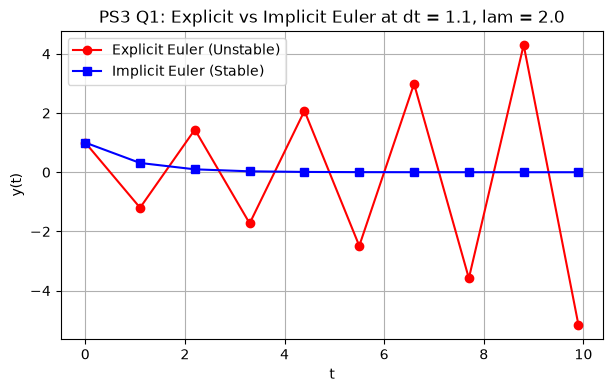
\includegraphics[width=0.72\linewidth]{Linear_Ordinary_Differential_Equations__04_Linear_ODE_Problem_Set_Solutions__c2_o0.png}
\end{center}

\subsection{Second-Order ODEs: Harmonic Oscillator, Timescales \& RK4}
For a damped oscillator $m\ddot x + \gamma\dot x + kx = 0$, define $b = \frac{\gamma}{2m}$, $\omega_0 = \sqrt{\frac{k}{m}}$, and damping ratio $\zeta = \frac{b}{\omega_0} = \frac{\gamma}{2\sqrt{km}}$. Substituting $x = e^{rt}$ gives $r^2 + 2br + \omega_0^2 = 0 \implies r = -b \pm \sqrt{b^2 - \omega_0^2}$.

\begin{center}
\begin{tabularx}{\linewidth}{@{}>{\raggedright\arraybackslash}p{0.20\linewidth}
  >{\centering\arraybackslash}p{0.18\linewidth}
  >{\raggedright\arraybackslash}X@{}}
\toprule
\rowcolor{accent!10}
\textbf{Regime} & \textbf{Condition} & \textbf{Solution \& Behaviour} \\
\midrule
Underdamped & $b^2 < \omega_0^2$ ($\zeta < 1$) & $x = e^{-bt}(A\cos\omega_d t + B\sin\omega_d t)$, $\omega_d=\sqrt{\omega_0^2-b^2}$ (oscillates \& decays) \\
Critically damped & $b^2 = \omega_0^2$ ($\zeta = 1$) & $x = (A + Bt)e^{-bt}$ (fastest decay without oscillation) \\
Overdamped & $b^2 > \omega_0^2$ ($\zeta > 1$) & $x = Ae^{r_1 t} + Be^{r_2 t}$, $r_{1,2} = -b \pm \sqrt{b^2-\omega_0^2}$ (slow, non-oscillatory) \\
\bottomrule
\end{tabularx}
\end{center}

\begin{center}
\begin{tikzpicture}[x=0.72cm,y=1.45cm,>=Stealth]
  \draw[->] (0,0)--(9.2,0) node[right] {\small $t$};
  \draw[->] (0,-1.15)--(0,1.25) node[above] {\small $x$};
  \draw[thick,navy,domain=0:8.8,samples=160]
    plot (\x,{exp(-0.22*\x)*cos(2*\x r)});
  \draw[thick,teal,domain=0:8.8,samples=80]
    plot (\x,{(1+0.7*\x)*exp(-0.7*\x)});
  \draw[thick,rust,domain=0:8.8,samples=80]
    plot (\x,{1.6*exp(-0.35*\x)-0.6*exp(-1.8*\x)});
  \node[navy] at (6.6,0.95) {\small underdamped};
  \node[teal] at (6.6,0.5) {\small critical};
  \node[rust] at (6.6,-0.6) {\small overdamped};
\end{tikzpicture}
\end{center}

\begin{derivbox}[1st-Order System Conversion, Energy Decay \& Overdamped Reduction (PS II Q1)]
\begin{itemize}
\item \textbf{Convert to 1st-Order System:} Set $y_0 = x$ and $y_1 = v = \dot x$:
\[
\frac{\dd y_0}{\dd t} = y_1,\qquad \frac{\dd y_1}{\dd t} = -\frac{\gamma}{m}y_1 - \frac{k}{m}y_0 + \frac{F(t)}{m}.
\]
\item \textbf{Energy Decay:} With $E = \frac{1}{2}m\dot x^2 + \frac{1}{2}kx^2$, differentiating gives $\frac{\dd E}{\dd t} = \dot x(m\ddot x + kx) = -\gamma \dot x^2 \le 0$.
\item \textbf{Why Simple Euler Fails on Undamped SHM ($\gamma = 0$):} Simple Euler updates $x_{n+1} = x_n + v_n \Delta t$ and $v_{n+1} = v_n - \frac{k}{m}x_n \Delta t$, which adds artificial energy every step ($E_{n+1} > E_n$) and spirals outward. \textbf{Euler-Cromer} fixes this by using the \emph{new} velocity: $v_{n+1} = v_n - \frac{k}{m}x_n\Delta t$, then $x_{n+1} = x_n + v_{n+1}\Delta t$.
\item \textbf{Overdamped Reduction (PS II Q1):} Characteristic timescales are $\tau_{\text{osc}} = \sqrt{m/k}$, $\tau_{\text{damp}} = \gamma/k$, $\tau_{\text{diss}} = m/\gamma$. When viscous damping dominates inertia ($\gamma^2 \gg mk$), drop $m\ddot x$: $\gamma\dot x + kx = A\sin(\omega t)$. (In PS II Q1: $m=0.5,\gamma=1,k=1,\omega=2\pi$, so $\gamma^2 = 1$ is comparable to $mk = 0.5$ and $\omega$ is fast; inertia matters at early times!)
\end{itemize}
\end{derivbox}

\begin{keybox}[Runge-Kutta 4th Order (RK4) for $\dot{\mathbf{y}} = \mathbf{f}(t, \mathbf{y})$]
Evaluate 4 slopes per step ($\Delta t = h$); local error $O(h^5)$, global error $O(h^4)$:
\[
\begin{aligned}
\mathbf{k}_1 &= \mathbf{f}(t_n, \mathbf{y}_n), &
\mathbf{k}_2 &= \mathbf{f}\!\left(t_n + \tfrac{h}{2},\, \mathbf{y}_n + \tfrac{h}{2}\mathbf{k}_1\right), \\
\mathbf{k}_3 &= \mathbf{f}\!\left(t_n + \tfrac{h}{2},\, \mathbf{y}_n + \tfrac{h}{2}\mathbf{k}_2\right), &
\mathbf{k}_4 &= \mathbf{f}(t_n + h,\, \mathbf{y}_n + h\mathbf{k}_3),
\end{aligned}
\qquad
\mathbf{y}_{n+1} = \mathbf{y}_n + \frac{h}{6}(\mathbf{k}_1 + 2\mathbf{k}_2 + 2\mathbf{k}_3 + \mathbf{k}_4).
\]
\end{keybox}

\begin{jupytercode}[Undamped SHM: Simple Euler Energy Blowup vs Euler-Cromer]
import numpy as np
import matplotlib.pyplot as plt

# Undamped SHM (gamma = 0): Simple Euler blows up vs Euler-Cromer stays bounded
k, m = 1.0, 1.0
dt = 0.1
t = np.arange(0, 40 + dt, dt)
n = len(t)

x_eu = np.zeros(n); v_eu = np.zeros(n)
x_ec = np.zeros(n); v_ec = np.zeros(n)
x_eu[0], v_eu[0] = 1.0, 0.0
x_ec[0], v_ec[0] = 1.0, 0.0

for i in range(n - 1):
    # Simple Euler (uses old v to update x)
    x_eu[i + 1] = x_eu[i] + v_eu[i] * dt
    v_eu[i + 1] = v_eu[i] - (k / m) * x_eu[i] * dt

    # Euler-Cromer (updates v first, then uses NEW v for x)
    v_ec[i + 1] = v_ec[i] - (k / m) * x_ec[i] * dt
    x_ec[i + 1] = x_ec[i] + v_ec[i + 1] * dt

plt.figure(figsize=(8, 4))
plt.plot(t, x_eu, 'r--', label='Simple Euler (Energy grows)')
plt.plot(t, x_ec, 'b-', label='Euler-Cromer (Stable amplitude)')
plt.xlabel('Time')
plt.ylabel('Position x(t)')
plt.title('Undamped SHM: Simple Euler vs Euler-Cromer')
plt.legend()
plt.grid(True)
plt.show()
\end{jupytercode}
\begin{center}
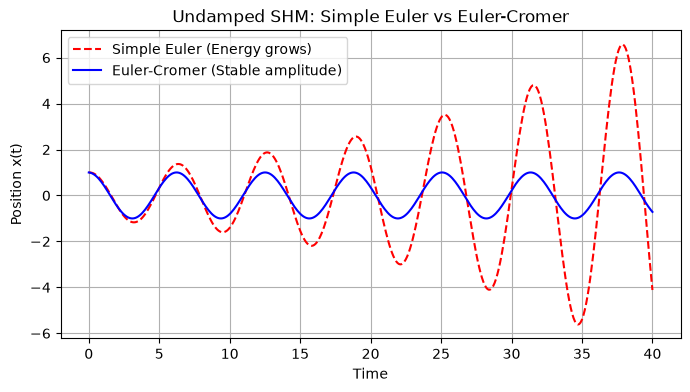
\includegraphics[width=0.75\linewidth]{Linear_Ordinary_Differential_Equations__02_Second_Order_ODEs_SHM_and_RK4__c1_o0.png}
\end{center}

\begin{jupytercode}[Professor's Exact Code: Damped SHM with RK4 (Notes/SHM\_rk4.ipynb)]
import numpy as np
import matplotlib.pyplot as plt

k = 1                 # spring constant
m = 1                 # mass
gamma = 0.1           # damping coefficient
t_end = 100           # final time
dt = 0.1              # time step
y0 = np.array([1, 0]) # initial conditions: position, velocity

t = np.arange(0, t_end + dt, dt)  # time vector, including t_end
n = len(t)

y = np.zeros((2, n))              # solution matrix: row 0 = position, row 1 = velocity
y[:, 0] = y0                      # set initial conditions

for i in range(n - 1):
    k1 = np.array([
        y[1, i],
        -(gamma / m * y[1, i] + k / m * y[0, i])
    ])

    k2 = np.array([
        y[1, i] + 0.5 * dt * k1[1],
        -k / m * (y[0, i] + 0.5 * dt * k1[0])
        - gamma / m * (y[1, i] + 0.5 * dt * k1[1])
    ])

    k3 = np.array([
        y[1, i] + 0.5 * dt * k2[1],
        -k / m * (y[0, i] + 0.5 * dt * k2[0])
        - gamma / m * (y[1, i] + 0.5 * dt * k2[1])
    ])

    k4 = np.array([
        y[1, i] + dt * k3[1],
        -k / m * (y[0, i] + dt * k3[0])
        - gamma / m * (y[1, i] + dt * k3[1])
    ])

    # update solution
    y[:, i + 1] = y[:, i] + dt * (k1 + 2 * k2 + 2 * k3 + k4) / 6

plt.plot(t, y[0, :])
plt.xlabel("Time")
plt.ylabel("Position")
plt.grid(True)
plt.show()
\end{jupytercode}
\begin{center}
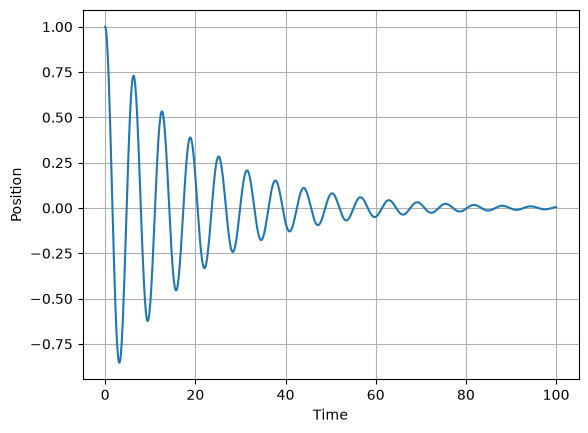
\includegraphics[width=0.72\linewidth]{Linear_Ordinary_Differential_Equations__02_Second_Order_ODEs_SHM_and_RK4__c3_o0.png}
\end{center}

\begin{jupytercode}[Exact Class Code: Simple vs Improved Euler SHM (Simple Harmonic Ocilator.ipynb)]
import numpy as np
import matplotlib.pyplot as plt

def simple_euler_shm(x0, v0, k, m, dt, t_total):
    t = np.arange(0, t_total, dt)
    x = np.zeros(len(t))
    v = np.zeros(len(t))
    x[0], v[0] = x0, v0
    for i in range(len(t) - 1):
        x[i + 1] = x[i] + v[i] * dt
        v[i + 1] = v[i] - (k / m) * x[i] * dt
    return t, x, v

def improved_euler_shm(x0, v0, k, m, dt, t_total):
    t = np.arange(0, t_total, dt)
    x = np.zeros(len(t))
    v = np.zeros(len(t))
    x[0], v[0] = x0, v0
    for i in range(len(t) - 1):
        x_mid = x[i] + v[i] * dt / 2
        v_mid = v[i] - (k / m) * x[i] * dt / 2
        x[i + 1] = x[i] + v_mid * dt
        v[i + 1] = v[i] - (k / m) * x_mid * dt
    return t, x, v

t1, x1, v1 = simple_euler_shm(1, 0, 1, 1, 0.1, 30)
t2, x2, v2 = improved_euler_shm(1, 0, 1, 1, 0.1, 30)

plt.figure(figsize=(8, 4))
plt.plot(t1, x1, '--', label='Simple Euler')
plt.plot(t2, x2, '-', label='Improved Euler')
plt.xlabel('Time')
plt.ylabel('Position')
plt.title('Class Code: Simple vs Improved Euler on SHM')
plt.legend()
plt.grid(True)
plt.show()
\end{jupytercode}
\begin{center}
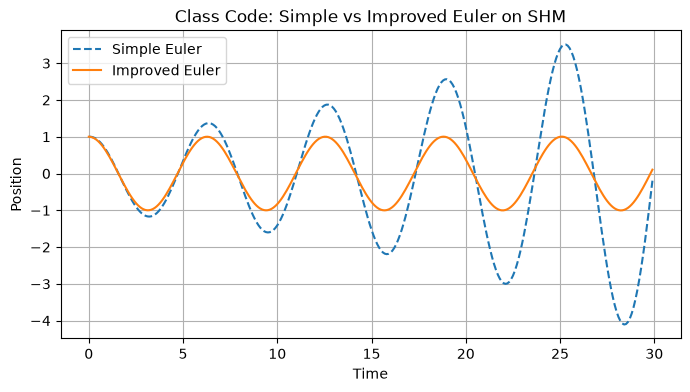
\includegraphics[width=0.75\linewidth]{Linear_Ordinary_Differential_Equations__02_Second_Order_ODEs_SHM_and_RK4__c5_o0.png}
\end{center}

\begin{jupytercode}[Problem Set II Q1: Driven 2nd-Order Oscillator vs Overdamped Approximation (RK4)]
import numpy as np
import matplotlib.pyplot as plt

# Full 2nd-order system vs Overdamped 1st-order reduction using RK4
m, gamma, k, A = 0.5, 1.0, 1.0, 1.0
omega = 2 * np.pi
dt = 0.01
t = np.arange(0, 10 + dt, dt)
n = len(t)

# Full system: y[0] = x, y[1] = v
y = np.zeros((2, n))
y[:, 0] = [3.0, 5.0]

# Reduced 1st-order system: gamma * x_dot + k * x = A * sin(omega * t)
x_red = np.zeros(n)
x_red[0] = 3.0

def f_full(t_val, state):
    x_val, v_val = state[0], state[1]
    return np.array([v_val, (A * np.sin(omega * t_val) - gamma * v_val - k * x_val) / m])

def f_red(t_val, x_val):
    return (A * np.sin(omega * t_val) - k * x_val) / gamma

for i in range(n - 1):
    k1 = f_full(t[i], y[:, i])
    k2 = f_full(t[i] + 0.5*dt, y[:, i] + 0.5*dt*k1)
    k3 = f_full(t[i] + 0.5*dt, y[:, i] + 0.5*dt*k2)
    k4 = f_full(t[i] + dt, y[:, i] + dt*k3)
    y[:, i + 1] = y[:, i] + dt * (k1 + 2*k2 + 2*k3 + k4) / 6

    r1 = f_red(t[i], x_red[i])
    r2 = f_red(t[i] + 0.5*dt, x_red[i] + 0.5*dt*r1)
    r3 = f_red(t[i] + 0.5*dt, x_red[i] + 0.5*dt*r2)
    r4 = f_red(t[i] + dt, x_red[i] + dt*r3)
    x_red[i + 1] = x_red[i] + dt * (r1 + 2*r2 + 2*r3 + r4) / 6

plt.figure(figsize=(8, 4))
plt.plot(t, y[0], 'b-', label='Full 2nd-order')
plt.plot(t, x_red, 'r--', label='Overdamped 1st-order (m=0)')
plt.xlabel('t')
plt.ylabel('x(t)')
plt.title('PS2 Q1: Driven Oscillator vs Overdamped Approximation')
plt.legend()
plt.grid(True)
plt.show()
\end{jupytercode}
\begin{center}
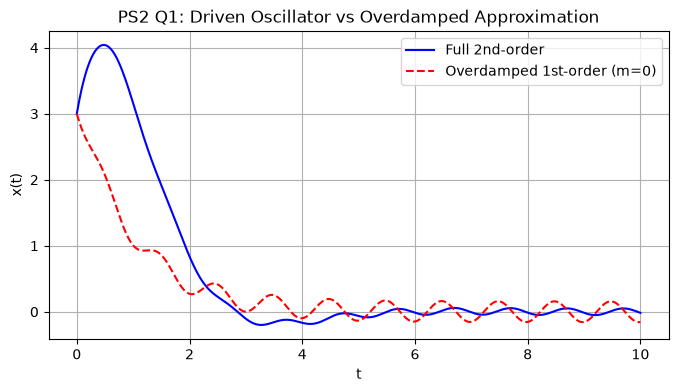
\includegraphics[width=0.75\linewidth]{Linear_Ordinary_Differential_Equations__04_Linear_ODE_Problem_Set_Solutions__c4_o0.png}
\end{center}

\subsection{2D Linear Autonomous Systems ($\dot{\mathbf{X}} = J\mathbf{X}$)}
For $\dot{X} = J X$ with $X = \binom{u}{v}$ and $J = \begin{pmatrix} a & b \\ c & d \end{pmatrix}$, substituting $X = \mathbf{v}e^{\lambda t}$ gives $\det(J - \lambda I) = 0$:
\[
\lambda^2 - \tau\lambda + \Delta = 0, \qquad \tau = \operatorname{tr}J = a+d, \qquad \Delta = \det J = ad-bc, \qquad \lambda_{1,2} = \frac{\tau \pm \sqrt{\tau^2 - 4\Delta}}{2}.
\]

\begin{center}
\begin{tabularx}{\linewidth}{@{}>{\centering\arraybackslash}p{0.09\linewidth}
  >{\centering\arraybackslash}p{0.09\linewidth}
  >{\centering\arraybackslash}p{0.16\linewidth}
  >{\raggedright\arraybackslash}X@{}}
\toprule
\rowcolor{accent!10}
$\Delta$ & $\tau$ & Discriminant & Fixed-Point Type (and PS II Q3 Examples) \\
\midrule
$<0$ & any & any & \textbf{Saddle} (1 positive, 1 negative $\lambda$); e.g. Q3(iii) $\begin{pmatrix}1&0\\0&-1\end{pmatrix}$, $\lambda = 1,-1$ \\
$>0$ & $<0$ & $\tau^2 - 4\Delta \ge 0$ & \textbf{Stable node} (both real $\lambda < 0$); e.g. Q3(ii) $\begin{pmatrix}-1&0\\0&-1\end{pmatrix}$, $\lambda = -1,-1$ \\
$>0$ & $<0$ & $\tau^2 - 4\Delta < 0$ & \textbf{Stable spiral} (complex $\alpha \pm i\beta, \alpha < 0$); e.g. Q3(v) $\lambda = -0.5 \pm 0.866i$ \\
$>0$ & $>0$ & $\tau^2 - 4\Delta \ge 0$ & \textbf{Unstable node} (both real $\lambda > 0$); e.g. Q3(i) $\begin{pmatrix}1&0\\0&1\end{pmatrix}$, $\lambda = 1,1$ \\
$>0$ & $>0$ & $\tau^2 - 4\Delta < 0$ & \textbf{Unstable spiral} (complex $\alpha \pm i\beta, \alpha > 0$); e.g. Q3(iv) $\lambda = 0.5 \pm 0.866i$ \\
$>0$ & $0$ & $\tau^2 - 4\Delta < 0$ & \textbf{Center} (pure imaginary $\pm i\beta$); e.g. Q3(vi) $\begin{pmatrix}0&-1\\1&0\end{pmatrix}$, $\lambda = \pm i$ \\
\bottomrule
\end{tabularx}
\end{center}

\begin{warnbox}[Why Simple Euler Fails on Centers (PS II Q3(vi))]
For a center ($\lambda = \pm i\beta$), Simple Euler updates $X_{n+1} = (I + \Delta t J)X_n$, whose amplification eigenvalues are $\mu = 1 \pm i\beta\Delta t$. Their magnitude is $|\mu| = \sqrt{1 + \beta^2\Delta t^2} > 1$ for \textbf{any} $\Delta t > 0$, so trajectories spiral outward instead of forming closed circles. RK4 keeps $|\mu| \approx 1$ and preserves closed orbits.
\end{warnbox}

\begin{jupytercode}[2D Linear System: Stable Spiral Phase Portrait with RK4]
import numpy as np
import matplotlib.pyplot as plt

# Example 1: Stable Spiral -> J = [[-0.2, 1], [-1, -0.2]]
J = np.array([[-0.2, 1.0],
              [-1.0, -0.2]])
eigvals, eigvecs = np.linalg.eig(J)
print('Eigenvalues:', eigvals)

dt = 0.05
t = np.arange(0, 20, dt)
n = len(t)
X = np.zeros((2, n))
X[:, 0] = [1.0, 0.5]

for i in range(n - 1):
    k1 = J @ X[:, i]
    k2 = J @ (X[:, i] + 0.5 * dt * k1)
    k3 = J @ (X[:, i] + 0.5 * dt * k2)
    k4 = J @ (X[:, i] + dt * k3)
    X[:, i + 1] = X[:, i] + dt * (k1 + 2*k2 + 2*k3 + k4) / 6

plt.figure(figsize=(5, 5))
plt.plot(X[0], X[1], 'b-', label='Trajectory')
plt.plot(X[0, 0], X[1, 0], 'go', label='Start')
plt.plot(0, 0, 'rx', markersize=10, label='Fixed point (0,0)')
plt.xlabel('u')
plt.ylabel('v')
plt.title('Phase Portrait: Stable Spiral')
plt.legend()
plt.grid(True)
plt.axis('equal')
plt.show()
\end{jupytercode}
\begin{outbox}[Printed Output]
\texttt{Eigenvalues: [-0.2+1.j -0.2-1.j]}
\end{outbox}
\begin{center}
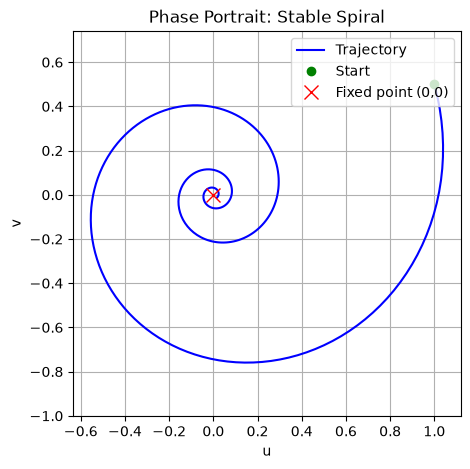
\includegraphics[width=0.52\linewidth]{Linear_Ordinary_Differential_Equations__03_2D_Linear_Autonomous_Systems__c1_o1.png}
\end{center}

\begin{jupytercode}[2D Center: Simple Euler Drifts Out vs RK4 Stays Closed]
import numpy as np
import matplotlib.pyplot as plt

# Example 2: Center -> J = [[0, 1], [-1, 0]] (Simple Euler spirals out, RK4 stays closed)
J_center = np.array([[0.0, 1.0],
                     [-1.0, 0.0]])
print('Center Eigenvalues:', np.linalg.eigvals(J_center))

dt = 0.1
t = np.arange(0, 20, dt)
n = len(t)

X_eu = np.zeros((2, n))
X_rk = np.zeros((2, n))
X_eu[:, 0] = [1.0, 0.0]
X_rk[:, 0] = [1.0, 0.0]

for i in range(n - 1):
    # Simple Euler
    X_eu[:, i + 1] = X_eu[:, i] + dt * (J_center @ X_eu[:, i])
    # RK4
    k1 = J_center @ X_rk[:, i]
    k2 = J_center @ (X_rk[:, i] + 0.5 * dt * k1)
    k3 = J_center @ (X_rk[:, i] + 0.5 * dt * k2)
    k4 = J_center @ (X_rk[:, i] + dt * k3)
    X_rk[:, i + 1] = X_rk[:, i] + dt * (k1 + 2*k2 + 2*k3 + k4) / 6

plt.figure(figsize=(5, 5))
plt.plot(X_eu[0], X_eu[1], 'r--', label='Simple Euler (Drifts out)')
plt.plot(X_rk[0], X_rk[1], 'b-', label='RK4 (Closed orbit)')
plt.xlabel('u')
plt.ylabel('v')
plt.title('Center: Why Simple Euler Fails')
plt.legend()
plt.grid(True)
plt.axis('equal')
plt.show()
\end{jupytercode}
\begin{outbox}[Printed Output]
\texttt{Center Eigenvalues: [0.+1.j 0.-1.j]}
\end{outbox}
\begin{center}
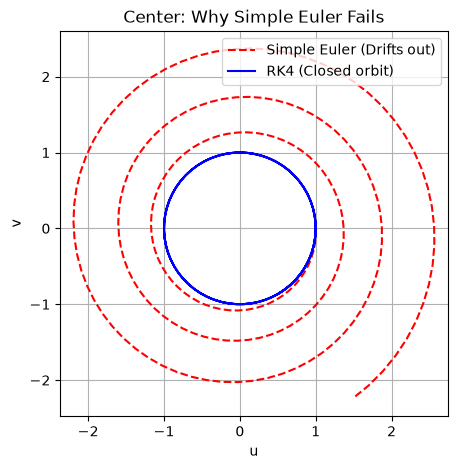
\includegraphics[width=0.52\linewidth]{Linear_Ordinary_Differential_Equations__03_2D_Linear_Autonomous_Systems__c2_o1.png}
\end{center}

\begin{jupytercode}[Problem Set II Q3: Eigenvalues, Spiral/Saddle Plots \& Center Test (All 6 Cases)]
import numpy as np
import matplotlib.pyplot as plt

# Eigenvalues and eigenvectors for all 6 matrices in Problem Set II Q3
# J = [[a, b], [c, d]] from Problem Set II Q3 (i)-(vi)
matrices = {
    '(i)':   np.array([[ 1,  0], [ 0,  1]]),   # a=d=1, b=c=0
    '(ii)':  np.array([[-1,  0], [ 0, -1]]),   # a=d=-1, b=c=0
    '(iii)': np.array([[ 1,  0], [ 0, -1]]),   # a=1, d=-1, b=c=0
    '(iv)':  np.array([[ 0,  1], [-1,  1]]),   # a=0, b=1, c=-1, d=1
    '(v)':   np.array([[ 0,  1], [-1, -1]]),   # a=0, b=1, c=-1, d=-1
    '(vi)':  np.array([[ 0, -1], [ 1,  0]])    # a=d=0, b=-1, c=1
}

for label in matrices:
    J = matrices[label]
    vals, vecs = np.linalg.eig(J)
    print(label, 'Eigenvalues:', np.round(vals, 3))

# Simple phase portrait check for (v) Stable Spiral and (iii) Saddle
def run_rk4(J, X0, t_end=4.0, dt=0.05):
    t = np.arange(0, t_end, dt)
    X = np.zeros((2, len(t)))
    X[:, 0] = X0
    for i in range(len(t) - 1):
        k1 = J @ X[:, i]
        k2 = J @ (X[:, i] + 0.5 * dt * k1)
        k3 = J @ (X[:, i] + 0.5 * dt * k2)
        k4 = J @ (X[:, i] + dt * k3)
        X[:, i + 1] = X[:, i] + dt * (k1 + 2*k2 + 2*k3 + k4) / 6
    return X

X_spiral = run_rk4(matrices['(v)'],   [1.0, 0.5], t_end=8.0)
X_saddle = run_rk4(matrices['(iii)'], [0.3, 1.5], t_end=1.8)

plt.figure(figsize=(10, 4))
plt.subplot(1, 2, 1)
plt.plot(X_spiral[0], X_spiral[1], 'b-')
plt.plot(0, 0, 'rx')
plt.title('(v) Stable Spiral')
plt.xlabel('u'); plt.ylabel('v'); plt.grid(True)

plt.subplot(1, 2, 2)
plt.plot(X_saddle[0], X_saddle[1], 'r-')
plt.plot(0, 0, 'rx')
plt.title('(iii) Saddle Point')
plt.xlabel('u'); plt.ylabel('v'); plt.grid(True)
plt.tight_layout()
plt.show()

# Q3 (vi): Center J = [[0, -1], [1, 0]] -> Simple Euler vs RK4
J_vi = matrices['(vi)']
dt = 0.08
t = np.arange(0, 12.0, dt)
n = len(t)

X_eu = np.zeros((2, n))
X_rk = run_rk4(J_vi, [1.0, 0.0], t_end=12.0, dt=dt)
X_eu[:, 0] = [1.0, 0.0]

for i in range(n - 1):
    X_eu[:, i + 1] = X_eu[:, i] + dt * (J_vi @ X_eu[:, i])

plt.figure(figsize=(5, 5))
plt.plot(X_eu[0], X_eu[1], 'r--', label='Simple Euler (Spirals out)')
plt.plot(X_rk[0], X_rk[1], 'b-', label='RK4 (Closed circle)')
plt.xlabel('u'); plt.ylabel('v')
plt.title('Q3(vi) Center: Simple Euler vs RK4')
plt.legend(); plt.grid(True); plt.axis('equal'); plt.show()
\end{jupytercode}
\begin{outbox}[Printed Output (PS II Q3 Eigenvalues)]
\texttt{(i) Eigenvalues: [1.+0.j 1.+0.j] \quad (ii) [-1.+0.j -1.+0.j] \quad (iii) [ 1.+0.j -1.+0.j]}\\
\texttt{(iv) Eigenvalues: [0.5+0.866j 0.5-0.866j] \quad (v) [-0.5+0.866j -0.5-0.866j] \quad (vi) [0.+1.j 0.-1.j]}
\end{outbox}
\begin{center}
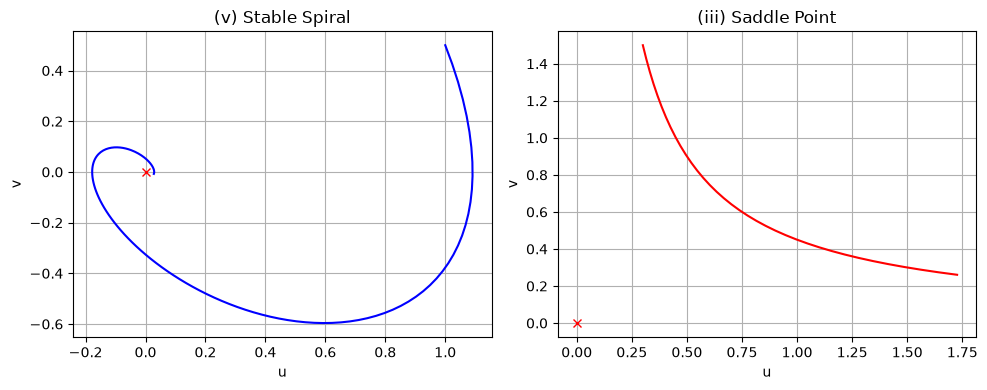
\includegraphics[width=0.58\linewidth]{Linear_Ordinary_Differential_Equations__04_Linear_ODE_Problem_Set_Solutions__c7_o0.png}\hfill
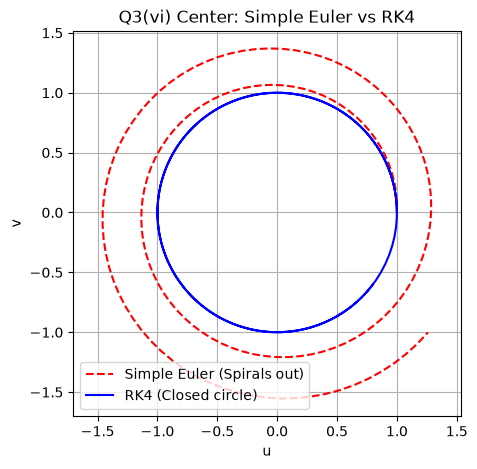
\includegraphics[width=0.39\linewidth]{Linear_Ordinary_Differential_Equations__04_Linear_ODE_Problem_Set_Solutions__c8_o0.png}
\end{center}

%============================================================
\clearpage
\colorlet{accent}{teal}
\section{Nonlinear Ordinary Differential Equations}
{\sloppy\small\emph{Notebooks covered: \texttt{01\_1D\_Nonlinear\_Flows\_and\_Bifurcations.ipynb}, \texttt{02\_2D\_Nonlinear\_Systems\_and\_Phase\_Plane.ipynb}, \texttt{03\_Nonlinear\_System\_Solvers\_Newton\_Method.ipynb}, \texttt{04\_Nonlinear\_ODE\_Problem\_Set\_Solutions.ipynb}. Sources: \texttt{lec10--11.pdf}, \texttt{Problem Set II Q2, Q4, Q5}, \texttt{Newton\_SOE.ipynb}.}\par}

\subsection{1D Flows, Fixed Points \& Linear Stability}
For a 1D autonomous ODE $\dot x = f(x)$, \textbf{fixed points} satisfy $f(x^*) = 0$. Perturbing $x = x^* + u$ and Taylor expanding gives $\dot u = f'(x^*)u \implies u(t) = u(0)e^{f'(x^*)t}$.

\begin{keybox}[1D Stability Criterion \& Graphical Test]
\[
\boxed{\;f'(x^*) < 0 \implies \text{Stable},\qquad f'(x^*) > 0 \implies \text{Unstable}\;}
\]
If $f'(x^*) = 0$, the linear test fails: plot $f(x)$ vs $x$ (arrows point right where $f>0$, left where $f<0$; downward crossing is stable, upward crossing is unstable).
\end{keybox}

\textbf{Double-Well Potential:} Gradient flow $\dot x = -V'(x)$ with $V(x) = -\frac{k}{2}x^2 + \frac{\lambda}{4}x^4$ ($k,\lambda>0$) gives $\dot x = kx - \lambda x^3 = x(k - \lambda x^2)$. Fixed points: $x^* = 0$ ($f'(0) = k > 0$, unstable) and $x^* = \pm\sqrt{k/\lambda}$ ($f'(\pm\sqrt{k/\lambda}) = -2k < 0$, stable).

\begin{warnbox}[Double-Well Sign Trap]
$V = -\frac{k}{2}x^2 + \frac{\lambda}{4}x^4$ has minima at $\pm\sqrt{k/\lambda}$. Reversing the signs to $+\frac{k}{2}x^2 - \frac{\lambda}{4}x^4$ is an inverted well with minimum at $0$.
\end{warnbox}

\begin{jupytercode}[1D Flow Plot: Pitchfork Bifurcation dx/dt = r*x - x\textasciicircum{}3]
import numpy as np
import matplotlib.pyplot as plt

# Graphical analysis: plot f(x) = r*x - x^3 before and after bifurcation
x_grid = np.linspace(-1.5, 1.5, 200)

plt.figure(figsize=(7, 4))
plt.plot(x_grid, -0.5 * x_grid - x_grid**3, 'b--', label='r = -0.5 (1 stable fixed point at 0)')
plt.plot(x_grid,  1.0 * x_grid - x_grid**3, 'r-',  label='r = +1.0 (0 unstable, +/-1 stable)')
plt.axhline(0, color='k', linewidth=0.8)
plt.xlabel('x')
plt.ylabel('dx/dt = f(x)')
plt.title('1D Pitchfork Bifurcation: dx/dt = r*x - x^3')
plt.legend()
plt.grid(True)
plt.show()
\end{jupytercode}
\begin{center}
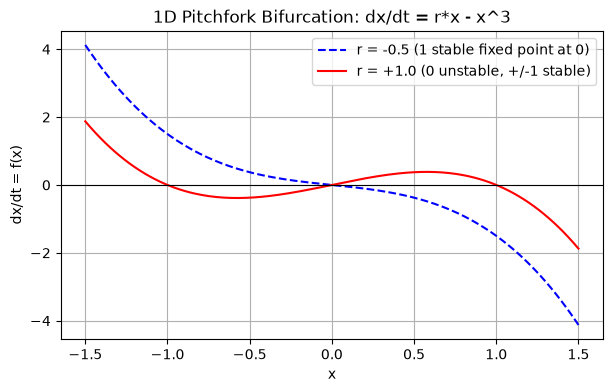
\includegraphics[width=0.70\linewidth]{Nonlinear_Ordinary_Differential_Equations__01_1D_Nonlinear_Flows_and_Bifurcations__c1_o0.png}
\end{center}

\begin{jupytercode}[1D Simple Euler Trajectories for dx/dt = x - x\textasciicircum{}3]
import numpy as np
import matplotlib.pyplot as plt

# Simple Euler time evolution for r = 1.0 from different starting points
r = 1.0
dt = 0.05
t = np.arange(0, 6, dt)
n = len(t)

plt.figure(figsize=(7, 4))
for x0 in [-1.4, -0.2, 0.2, 1.4]:
    x = np.zeros(n)
    x[0] = x0
    for i in range(n - 1):
        x[i + 1] = x[i] + dt * (r * x[i] - x[i]**3)
    plt.plot(t, x, label=f'x0 = {x0}')

plt.axhline( 1.0, color='gray', linestyle=':', label='x* = +/-1 (stable)')
plt.axhline(-1.0, color='gray', linestyle=':')
plt.axhline( 0.0, color='k', linestyle='--', alpha=0.5, label='x* = 0 (unstable)')
plt.xlabel('t')
plt.ylabel('x(t)')
plt.title('Simple Euler Trajectories for dx/dt = x - x^3')
plt.legend()
plt.grid(True)
plt.show()
\end{jupytercode}
\begin{center}
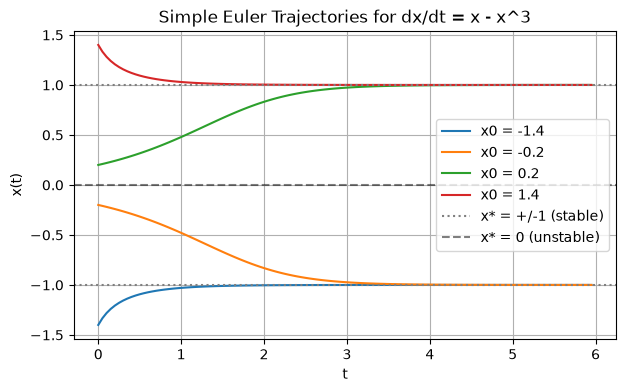
\includegraphics[width=0.70\linewidth]{Nonlinear_Ordinary_Differential_Equations__01_1D_Nonlinear_Flows_and_Bifurcations__c2_o0.png}
\end{center}

\begin{jupytercode}[Exam Note (Premid Fallback): 1D Newton Check for Transcendental Fixed Point]
import numpy as np

# Quick 1D Newton check to find non-zero fixed point of dx/dt = 1.3*x - ln(1 + x)
x_root = -0.5
for step in range(15):
    fx = 1.3 * x_root - np.log(1.0 + x_root)
    fpx = 1.3 - 1.0 / (1.0 + x_root)
    x_root = x_root - fx / fpx

print(f'Non-zero fixed point x* = {x_root:.6f}')
print(f'Check f(x*) = {1.3 * x_root - np.log(1.0 + x_root):.2e}')
\end{jupytercode}
\begin{outbox}[Printed Output]
\texttt{Non-zero fixed point x* = -0.422970 \quad | \quad Check f(x*) = 0.00e+00}
\end{outbox}

\subsection{1D Bifurcations \& Problem Set II Q2}
A bifurcation occurs when varying a parameter $r$ creates/destroys fixed points or flips their stability:
\begin{enumerate}
\item \textbf{Saddle-Node} ($\dot x = r + x^2$): two fixed points collide and annihilate as $r$ crosses $0$.
\item \textbf{Transcritical} ($\dot x = rx - x^2$): two fixed points cross and exchange stability at $r=0$.
\item \textbf{Pitchfork} ($\dot x = rx \pm x^3$): symmetry-breaking into 3 branches at $r=0$.
\end{enumerate}

\begin{keybox}[Problem Set II Q2 Summary]
\begin{itemize}
\item \textbf{Q2(i) $\dot x = rx + x^3 - x^5$:} Fixed points $x^* = 0$ and $x^2 = \frac{1 \pm \sqrt{1+4r}}{2}$ (real for $r \ge -1/4$). At $r = 0.4$: $x^* = 0$ is unstable ($f'(0)=0.4$), while $x^* = \pm\sqrt{(1+\sqrt{2.6})/2} \approx \pm 1.1429$ are stable.
\item \textbf{Q2(ii) Spruce Budworm:} $\dot x = \frac{2x}{5}(1 - \frac{x}{20}) - \frac{x^2}{1+x^2}$. Plot $f(x)$ vs $x$ to read non-zero roots and stability.
\item \textbf{Q2(iii) $\dot x = rx - \ln(1+x)$ ($x > -1$):} Transcritical bifurcation at $r = 1$ ($f'(0) = r - 1$).
\end{itemize}
\end{keybox}

\begin{jupytercode}[Problem Set II Q2(i): Subcritical Pitchfork with 5th-Order Saturation]
import numpy as np
import matplotlib.pyplot as plt

# Q2 (i): Numerical integration with Simple Euler at r = 0.4
r = 0.4
dt = 0.05
t = np.arange(0, 8, dt)
n = len(t)

x_pos = np.zeros(n); x_pos[0] = 0.5
x_neg = np.zeros(n); x_neg[0] = -0.5

for i in range(n - 1):
    x_pos[i + 1] = x_pos[i] + dt * (r * x_pos[i] + x_pos[i]**3 - x_pos[i]**5)
    x_neg[i + 1] = x_neg[i] + dt * (r * x_neg[i] + x_neg[i]**3 - x_neg[i]**5)

x_star = np.sqrt((1 + np.sqrt(1 + 4*r)) / 2)
print('Positive stable fixed point x* =', round(x_star, 4))
print('Final x(t) from +0.5:', round(x_pos[-1], 4))
print('Final x(t) from -0.5:', round(x_neg[-1], 4))

plt.figure(figsize=(7, 4))
plt.plot(t, x_pos, 'b-', label='x(0) = +0.5')
plt.plot(t, x_neg, 'r-', label='x(0) = -0.5')
plt.axhline( x_star, color='gray', linestyle='--', label=f'x* = +/-{x_star:.2f}')
plt.axhline(-x_star, color='gray', linestyle='--')
plt.xlabel('t')
plt.ylabel('x(t)')
plt.title('Q2(i): dx/dt = rx + x^3 - x^5 (r = 0.4)')
plt.legend()
plt.grid(True)
plt.show()
\end{jupytercode}
\begin{outbox}[Printed Output]
\texttt{Positive stable fixed point x* = 1.1429 \quad|\quad Final from +0.5: 1.1429 \quad|\quad Final from -0.5: -1.1429}
\end{outbox}
\begin{center}
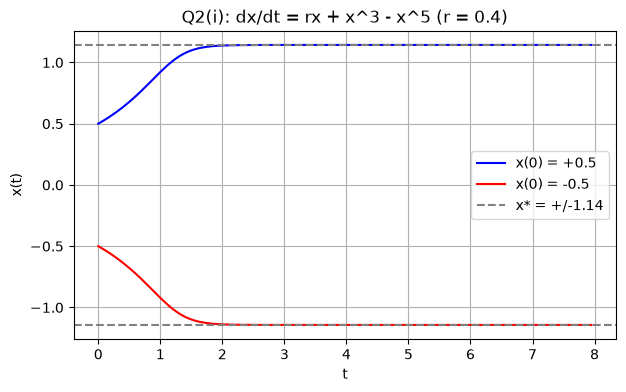
\includegraphics[width=0.70\linewidth]{Nonlinear_Ordinary_Differential_Equations__04_Nonlinear_ODE_Problem_Set_Solutions__c2_o1.png}
\end{center}

\begin{jupytercode}[Problem Set II Q2(ii): Spruce Budworm Flow Curve \& Trajectories]
import numpy as np
import matplotlib.pyplot as plt

# Q2 (ii): Plot f(x) to see fixed points and stability
x_grid = np.linspace(0, 20, 400)
f_budworm = 0.4 * x_grid * (1 - x_grid / 20) - (x_grid**2) / (1 + x_grid**2)

plt.figure(figsize=(7, 4))
plt.plot(x_grid, f_budworm, 'b-')
plt.axhline(0, color='k', linewidth=0.8)
plt.xlabel('x')
plt.ylabel('dx/dt')
plt.title('Q2(ii): Spruce Budworm Flow')
plt.grid(True)
plt.show()

# Check long-term trajectories from four initial values
dt = 0.1
t = np.arange(0, 60, dt)
plt.figure(figsize=(7, 4))
for x0 in [0.5, 2.0, 5.0, 18.0]:
    x = np.zeros(len(t))
    x[0] = x0
    for i in range(len(t) - 1):
        x[i + 1] = x[i] + dt * (0.4 * x[i] * (1 - x[i] / 20) - (x[i]**2) / (1 + x[i]**2))
    plt.plot(t, x, label=f'x(0) = {x0}')
plt.xlabel('t')
plt.ylabel('x(t)')
plt.title('Q2(ii): Time Evolution for Different Initial Conditions')
plt.legend()
plt.grid(True)
plt.show()
\end{jupytercode}
\begin{center}
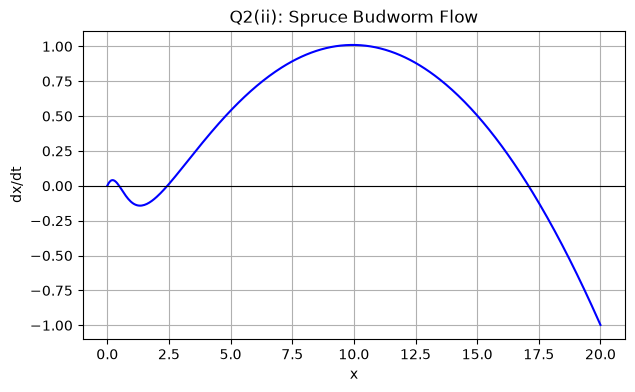
\includegraphics[width=0.48\linewidth]{Nonlinear_Ordinary_Differential_Equations__04_Nonlinear_ODE_Problem_Set_Solutions__c4_o0.png}\hfill
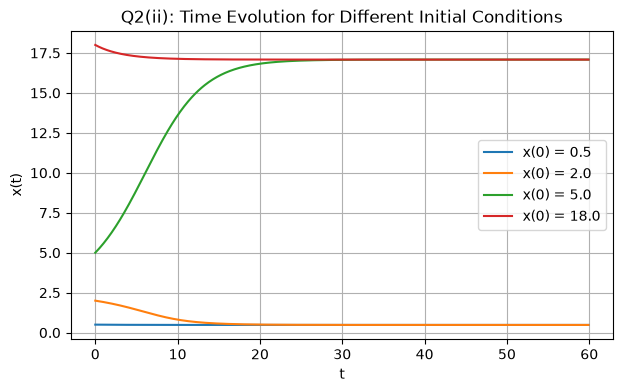
\includegraphics[width=0.48\linewidth]{Nonlinear_Ordinary_Differential_Equations__04_Nonlinear_ODE_Problem_Set_Solutions__c4_o1.png}
\end{center}

\begin{jupytercode}[Problem Set II Q2(iii): dx/dt = rx - ln(1 + x) Transcritical Bifurcation]
import numpy as np
import matplotlib.pyplot as plt

# Q2 (iii): Plot dx/dt = rx - ln(1 + x) for r < 1 and r > 1
x_grid = np.linspace(-0.7, 2.0, 300)

plt.figure(figsize=(7, 4))
plt.plot(x_grid, 0.7 * x_grid - np.log(1 + x_grid), 'b--', label='r = 0.7 (< 1): x*=0 stable')
plt.plot(x_grid, 1.3 * x_grid - np.log(1 + x_grid), 'r-',  label='r = 1.3 (> 1): x*=0 unstable')
plt.axhline(0, color='k', linewidth=0.8)
plt.xlabel('x')
plt.ylabel('dx/dt')
plt.title('Q2(iii): dx/dt = rx - ln(1+x) (Transcritical Bifurcation at r = 1)')
plt.legend()
plt.grid(True)
plt.show()
\end{jupytercode}
\begin{center}
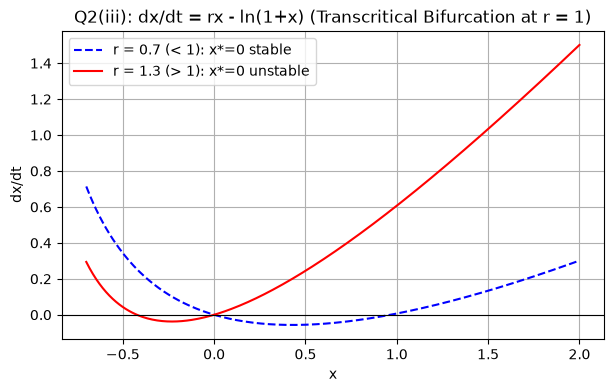
\includegraphics[width=0.70\linewidth]{Nonlinear_Ordinary_Differential_Equations__04_Nonlinear_ODE_Problem_Set_Solutions__c6_o0.png}
\end{center}

\subsection{Bead on a Rotating Hoop (Problem Set II Q5)}
A bead of mass $m$ moves on a vertical hoop of radius $r$ rotating at angular speed $\omega$:
\[
mr\ddot\varphi = -br\dot\varphi - mg\sin\varphi + mr\omega^2\sin\varphi\cos\varphi.
\]
\textbf{Fixed points ($\dot\varphi = \ddot\varphi = 0$):} $\sin\varphi\left(\omega^2\cos\varphi - \frac{g}{r}\right) = 0 \implies \varphi^* = 0, \pi$, plus $\varphi^* = \pm\arccos\!\left(\frac{g}{r\omega^2}\right)$ when $\omega^2 > \frac{g}{r}$.

\begin{keybox}[Pitchfork Bifurcation \& Overdamped Reduction (PS II Q5)]
\begin{itemize}
\item Critical speed $\omega_c^2 = \frac{g}{r}$. For $\omega^2 < \omega_c^2$, $\varphi^* = 0$ is stable; for $\omega^2 > \omega_c^2$, $\varphi^* = 0$ turns unstable and $\pm\varphi^*$ become stable (Supercritical Pitchfork).
\item \textbf{Overdamped Limit:} Viscous timescale $\tau = \frac{br}{mg}$; dropping $mr\ddot\varphi$ is valid when $\frac{m^2 g}{b^2 r} \ll 1$:
\[
br\dot\varphi = -mg\sin\varphi + mr\omega^2\sin\varphi\cos\varphi.
\]
\end{itemize}
\end{keybox}

\begin{center}
\begin{tikzpicture}[x=1.2cm,y=0.95cm,>=Stealth]
  \draw[->] (0,0)--(6.2,0) node[right] {\small $\omega^2$};
  \draw[->] (0,-2.0)--(0,2.1) node[above] {\small $\varphi^*$};
  \draw[very thick,teal] (0,0)--(3,0);
  \draw[thick,dashed,teal] (3,0)--(5.9,0);
  \draw[very thick,rust] (3,0) to[out=18,in=200] (5.9,1.7);
  \draw[very thick,rust] (3,0) to[out=-18,in=160] (5.9,-1.7);
  \draw[dashed] (3,-0.15)--(3,0.15);
  \node[below] at (3,-0.12) {\small $\omega_c^2=g/r$};
  \node[teal] at (1.45,0.3) {\small stable};
  \node[teal] at (4.5,-0.3) {\small unstable};
  \node[rust] at (4.6,1.4) {\small stable $\pm\varphi^*$};
\end{tikzpicture}
\end{center}

\begin{jupytercode}[Problem Set II Q5: Bead on Rotating Hoop (Full 2nd-Order vs Overdamped)]
import numpy as np
import matplotlib.pyplot as plt

# Q5: Compare Full 2nd-Order Hoop Equation vs Overdamped 1st-Order Approximation
m, b, omega, r, g = 1.0, 20.0, 5.0, 1.0, 9.8

ratio = (m**2 * g) / (b**2 * r)
print(f'Overdamped check (m^2*g / (b^2*r)) = {ratio:.4f} << 1')

dt = 0.005
t = np.arange(0, 6.0, dt)
n = len(t)

# Full system: phi and v = d(phi)/dt
phi_full = np.zeros(n); v_full = np.zeros(n)
phi_full[0] = 0.5; v_full[0] = 0.0

# Overdamped 1st-order system
phi_over = np.zeros(n)
phi_over[0] = 0.5

for i in range(n - 1):
    # Full 2nd-order Euler
    accel = (-b * r * v_full[i] - m * g * np.sin(phi_full[i])
             + m * r * (omega**2) * np.sin(phi_full[i]) * np.cos(phi_full[i])) / (m * r)
    v_full[i + 1] = v_full[i] + dt * accel
    phi_full[i + 1] = phi_full[i] + dt * v_full[i + 1]

    # Overdamped 1st-order Euler
    dphi = (-m * g * np.sin(phi_over[i])
            + m * r * (omega**2) * np.sin(phi_over[i]) * np.cos(phi_over[i])) / (b * r)
    phi_over[i + 1] = phi_over[i] + dt * dphi

phi_eq = np.arccos(g / (r * omega**2))
print(f'Analytical stable angle cos(phi) = g/(r*w^2) -> phi* = {phi_eq:.4f} rad')

plt.figure(figsize=(7, 4))
plt.plot(t, phi_full, 'b-', label='Full 2nd-order')
plt.plot(t, phi_over, 'r--', label='Overdamped 1st-order')
plt.axhline(phi_eq, color='gray', linestyle=':', label=f'Equilibrium ({phi_eq:.2f} rad)')
plt.xlabel('t')
plt.ylabel('phi(t)')
plt.title('Q5: Bead on Rotating Hoop')
plt.legend()
plt.grid(True)
plt.show()
\end{jupytercode}
\begin{outbox}[Printed Output]
\texttt{Overdamped check (m\textasciicircum{}2*g / (b\textasciicircum{}2*r)) = 0.0245 << 1 \quad|\quad phi* = 1.1680 rad}
\end{outbox}
\begin{center}
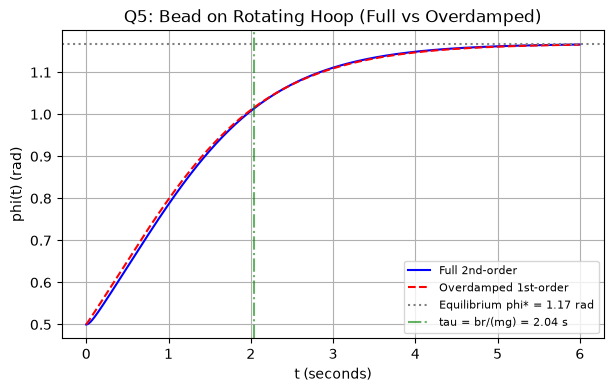
\includegraphics[width=0.70\linewidth]{Nonlinear_Ordinary_Differential_Equations__04_Nonlinear_ODE_Problem_Set_Solutions__c10_o1.png}
\end{center}

\subsection{2D Nonlinear Systems, Jacobian \& Phase Plane (Problem Set II Q4)}
Given $\dot x = f(x, y),\; \dot y = g(x, y)$:
\begin{enumerate}
\item Find fixed points $(x^*, y^*)$ where $f(x^*, y^*) = 0$ and $g(x^*, y^*) = 0$.
\item Compute the Jacobian matrix at each fixed point:
\[
J(x^*, y^*) = \begin{pmatrix} \frac{\partial f}{\partial x} & \frac{\partial f}{\partial y} \\[4pt] \frac{\partial g}{\partial x} & \frac{\partial g}{\partial y} \end{pmatrix}_{(x^*, y^*)}.
\]
\item Find eigenvalues $\lambda_1, \lambda_2$ (same table as 2D linear systems). Note: linearization is inconclusive if $\operatorname{Re}(\lambda) = 0$ (borderline center).
\end{enumerate}

\textbf{Lotka-Volterra Competition (PS II Q4):} $\dot x = x(3 - x - 2y)$, $\dot y = y(2 - y - x)$.
Fixed points: $(0,0)$ (unstable node, $\lambda=3,2$), $(1,1)$ (saddle, $\lambda = -1 \pm \sqrt{2}$), $(3,0)$ (stable node, $\lambda=-3,-1$), and $(0,2)$ (stable node, $\lambda=-1,-2$).

\begin{jupytercode}[2D Nonlinear System: Lotka-Volterra Predator-Prey (RK4 Phase Portrait)]
import numpy as np
import matplotlib.pyplot as plt

# Example: Lotka-Volterra Predator-Prey Model
# dx/dt = x - x*y,   dy/dt = -y + x*y
# Fixed points: (0, 0) [Saddle] and (1, 1) [Center]

def f_xy(x, y):
    return x - x * y, -y + x * y

# Check Jacobian at (1, 1): J = [[1 - y, -x], [y, -1 + x]] = [[0, -1], [1, 0]]
J_11 = np.array([[0, -1], [1, 0]])
print('Eigenvalues at (1, 1):', np.linalg.eigvals(J_11))

# Integrate two trajectories using RK4
dt = 0.02
t = np.arange(0, 12, dt)
n = len(t)

plt.figure(figsize=(5, 5))
for x0, y0 in [(1.5, 1.0), (2.2, 1.2)]:
    x = np.zeros(n); y = np.zeros(n)
    x[0], y[0] = x0, y0
    for i in range(n - 1):
        k1x, k1y = f_xy(x[i], y[i])
        k2x, k2y = f_xy(x[i] + 0.5*dt*k1x, y[i] + 0.5*dt*k1y)
        k3x, k3y = f_xy(x[i] + 0.5*dt*k2x, y[i] + 0.5*dt*k2y)
        k4x, k4y = f_xy(x[i] + dt*k3x, y[i] + dt*k3y)
        x[i + 1] = x[i] + dt * (k1x + 2*k2x + 2*k3x + k4x) / 6
        y[i + 1] = y[i] + dt * (k1y + 2*k2y + 2*k3y + k4y) / 6
    plt.plot(x, y, label=f'Start ({x0}, {y0})')

plt.plot(1, 1, 'ro', label='Center (1,1)')
plt.plot(0, 0, 'kx', label='Saddle (0,0)')
plt.xlabel('Prey x')
plt.ylabel('Predator y')
plt.title('Lotka-Volterra Phase Portrait (RK4)')
plt.legend()
plt.grid(True)
plt.show()
\end{jupytercode}
\begin{center}
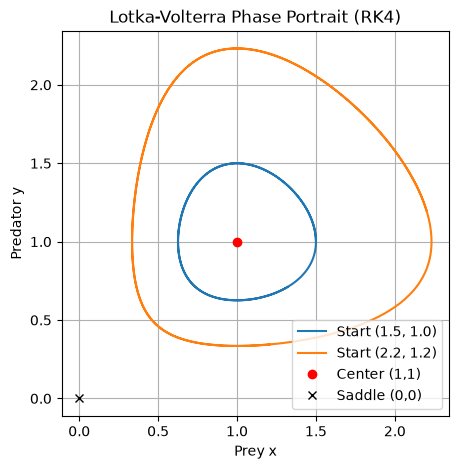
\includegraphics[width=0.52\linewidth]{Nonlinear_Ordinary_Differential_Equations__02_2D_Nonlinear_Systems_and_Phase_Plane__c1_o1.png}
\end{center}

\begin{jupytercode}[Problem Set II Q4: Competitive Exclusion Eigenvalues \& Phase Plane]
import numpy as np
import matplotlib.pyplot as plt

# Q4: Check Jacobian eigenvalues at all 4 fixed points
fixed_points = [(0, 0), (3, 0), (0, 2), (1, 1)]

for fp in fixed_points:
    x_s, y_s = fp
    J = np.array([[3 - 2*x_s - 2*y_s, -2*x_s],
                  [-y_s,               2 - 2*y_s - x_s]])
    vals = np.linalg.eigvals(J)
    print(f'Fixed point {fp}: eigenvalues = {np.round(vals, 3)}')

# Numerical phase plane with Simple Euler from several starting points
dt = 0.02
t = np.arange(0, 12, dt)
n = len(t)

plt.figure(figsize=(6, 5))
starts = [(0.4, 0.2), (2.0, 0.4), (0.3, 1.8), (2.5, 2.0), (1.2, 0.9), (0.8, 1.1)]
for x0, y0 in starts:
    x = np.zeros(n); y = np.zeros(n)
    x[0], y[0] = x0, y0
    for i in range(n - 1):
        dx = x[i] * (3 - x[i] - 2*y[i])
        dy = y[i] * (2 - y[i] - x[i])
        x[i + 1] = x[i] + dt * dx
        y[i + 1] = y[i] + dt * dy
    plt.plot(x, y, 'b-', alpha=0.7)
    plt.plot(x[0], y[0], 'go', markersize=5)

plt.plot([3, 0], [0, 2], 'ro', markersize=8, label='Stable: (3,0), (0,2)')
plt.plot([0, 1], [0, 1], 'kx', markersize=8, label='Unstable/Saddle: (0,0), (1,1)')
plt.xlabel('x')
plt.ylabel('y')
plt.title('Q4 Phase Plane (Simple Euler): Competitive Exclusion')
plt.legend()
plt.grid(True)
plt.show()
\end{jupytercode}
\begin{outbox}[Printed Output (PS II Q4)]
\texttt{FP (0, 0): [3. 2.] \quad|\quad FP (3, 0): [-3. -1.] \quad|\quad FP (0, 2): [-2. -1.] \quad|\quad FP (1, 1): [ 0.414 -2.414]}
\end{outbox}
\begin{center}
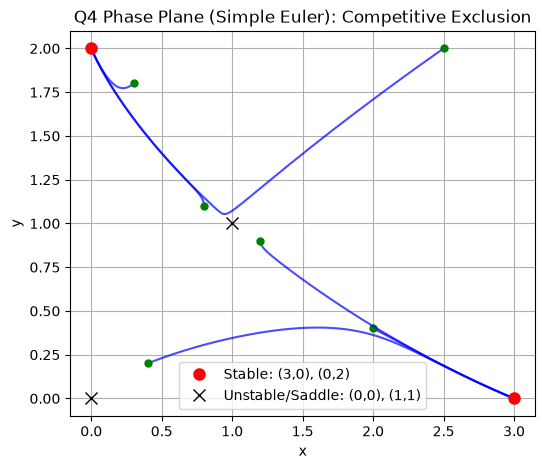
\includegraphics[width=0.60\linewidth]{Nonlinear_Ordinary_Differential_Equations__04_Nonlinear_ODE_Problem_Set_Solutions__c8_o1.png}
\end{center}

\subsection{Multivariable Newton-Raphson Solver}
To solve a coupled nonlinear system $\mathbf{F}(\mathbf{x}) = \mathbf{0}$ (such as finding 2D ODE fixed points), Taylor expansion $\mathbf{F}(\mathbf{x}_k + \Delta\mathbf{x}) \approx \mathbf{F}(\mathbf{x}_k) + J(\mathbf{x}_k)\Delta\mathbf{x} = \mathbf{0}$ gives quadratic convergence:
\[
\boxed{\;J(\mathbf{x}_k)\,\Delta\mathbf{x} = -\mathbf{F}(\mathbf{x}_k), \qquad \mathbf{x}_{k+1} = \mathbf{x}_k + \Delta\mathbf{x}\;}
\]

\begin{jupytercode}[Clean Multivariable Newton Solver (with np.linalg.solve)]
import numpy as np

# Simple class version (from 4/Newton_Systems.ipynb style)
# Solve:  x^2 + y^2 - 1 = 0  and  y - x^3 = 0

def F(x):
    return np.array([x[1] - x[0]**3,
                     x[0]**2 + x[1]**2 - 1.0])

def J(x):
    return np.array([[-3.0 * x[0]**2, 1.0],
                     [2.0 * x[0],     2.0 * x[1]]])

x = np.array([1.0, 2.0])  # initial guess
tol = 1e-8

for step in range(20):
    dx = np.linalg.solve(J(x), -F(x))
    x = x + dx
    if np.linalg.norm(dx) < tol:
        break

print(f'Converged in {step + 1} iterations')
print('Solution x =', np.round(x, 6))
print('Check F(x) =', np.round(F(x), 10))
\end{jupytercode}
\begin{outbox}[Printed Output]
\texttt{Converged in 6 iterations \quad|\quad Solution x = [0.826031 0.563624] \quad|\quad Check F(x) = [-0. 0.]}
\end{outbox}

\begin{jupytercode}[Exact Professor Code: Newton\_SOE.ipynb (Manual Gaussian Elimination Inside)]
import numpy as np

def func(x):
    return -1 * np.array([
        x[1] - x[0]**3,
        x[0]**2 + x[1]**2 - 1
    ])

# Initial guess
x = np.array([1.0, 2.0])

# Jacobian matrix
a = np.array([[-3 * x[0]**2, 1], [2 * x[0], 2 * x[1]]], dtype=float)

# Function vector
f = func(x)

# Number of variables
n = a.shape[0]

# Tolerance
tol = n * 1e-2

# Difference between successive x vectors
dx = np.ones(n)

while np.sum(dx) > tol:

    xprev = x.copy()

    # Gaussian elimination with partial pivoting
    for j in range(n - 1):

        # Find maximum element for pivoting
        I = j + np.argmax(np.abs(a[j:n, j]))

        # Row swapping
        if I != j:
            a[[j, I], :] = a[[I, j], :]
            f[[j, I]] = f[[I, j]]

        # Elimination
        for i in range(j + 1, n):

            # Multiplication factor
            mult = a[i, j] / a[j, j]

            for k in range(j, n):
                a[i, k] = a[i, k] - mult * a[j, k]

            f[i] = f[i] - mult * f[j]

    # Back substitution
    s = np.zeros(n)

    # Last variable
    s[n - 1] = f[n - 1] / a[n - 1, n - 1]

    x[n - 1] = x[n - 1] + s[n - 1]

    # Remaining variables
    for i in range(n - 2, -1, -1):

        SUM = 0.0

        for j in range(i + 1, n):
            SUM = SUM + a[i, j] * s[j]

        s[i] = (f[i] - SUM) / a[i, i]

        x[i] = x[i] + s[i]

    # Update Jacobian
    a = np.array([
        [-3 * x[0]**2, 1],
        [2 * x[0], 2 * x[1]]
    ], dtype=float)

    # Update function vector
    f = func(x)

    # Calculate difference between iterations
    dx = np.abs(xprev - x)

# Display solution
print("Solution:")
print(x)
\end{jupytercode}
\begin{outbox}[Printed Output]
\texttt{Solution: [0.82604011 0.56361977]}
\end{outbox}

%============================================================
\clearpage
\colorlet{accent}{violet}
\section{Linear Partial Differential Equations}
{\sloppy\small\emph{Notebooks covered: \texttt{01\_1D\_Diffusion\_Explicit\_FTCS.ipynb} to \texttt{06\_Linear\_PDE\_Problem\_Set\_Solutions.ipynb}. Sources: \texttt{lec\_pde.pdf}, \texttt{Tutorial\_03\_11\_26.pptx}, \texttt{problem\_set\_III Q2--Q6}, \texttt{1D\_diffusion.ipynb}, \texttt{1storderwaveeqn.ipynb}, \texttt{2ndorderwaveeqn.ipynb}.}\par}

\subsection{Finite Differences, Symmetries \& Boundary Conditions}
Grid points: $x_i = i\Delta x$ ($i = 0, \dots, N$, $L = N\Delta x$), $t_n = n\Delta t$.

\begin{center}
\begin{tabularx}{\linewidth}{@{}>{\raggedright\arraybackslash}p{0.23\linewidth}
  >{\raggedright\arraybackslash}X
  >{\centering\arraybackslash}p{0.13\linewidth}@{}}
\toprule
\rowcolor{accent!10}
\textbf{Derivative} & \textbf{Finite-Difference Formula} & \textbf{Error} \\
\midrule
Forward 1st & $f_i' \approx \dfrac{f_{i+1}-f_i}{\Delta x}$ & $O(\Delta x)$ \\
Backward 1st & $f_i' \approx \dfrac{f_i-f_{i-1}}{\Delta x}$ & $O(\Delta x)$ \\
Central 1st & $f_i' \approx \dfrac{f_{i+1}-f_{i-1}}{2\Delta x}$ & $O(\Delta x^2)$ \\
Central 2nd & $f_i'' \approx \dfrac{f_{i+1}-2f_i+f_{i-1}}{\Delta x^2} = \dfrac{1}{\Delta x}\left[\dfrac{f_{i+1}-f_i}{\Delta x}-\dfrac{f_i-f_{i-1}}{\Delta x}\right]$ & $O(\Delta x^2)$ \\
\bottomrule
\end{tabularx}
\end{center}

\textbf{Symmetries:} Diffusion ($\partial_t\rho = D\partial_x^2\rho$) and 2nd-order wave ($\partial_t^2\psi = c^2\partial_x^2\psi$) have translational ($x\to x+a$) and parity ($x\to -x$) symmetry; 1st-order wave ($\partial_t\psi = -c\partial_x\psi$) breaks parity ($x\to -x$). Boundaries break translational symmetry and dictate the steady state.

\begin{center}
\begin{tabularx}{\linewidth}{@{}>{\raggedright\arraybackslash}p{0.20\linewidth}
  >{\raggedright\arraybackslash}p{0.28\linewidth}
  >{\raggedright\arraybackslash}X@{}}
\toprule
\rowcolor{accent!10}
\textbf{BC Type} & \textbf{Condition} & \textbf{Code Implementation \& Effect} \\
\midrule
Dirichlet & $\rho(0,t)=a,\ \rho(L,t)=b$ & \texttt{rho[0] = a; rho[-1] = b} (breaks particle conservation; steady state is linear) \\
Neumann (No-flux) & $\partial_x\rho = 0 \implies J = 0$ at ends & \texttt{rho[0] = rho[1]; rho[-1] = rho[-2]} (strictly conserves total mass $\int \rho\,\dd x$) \\
Periodic & $\rho(0,t) = \rho(L,t)$ & \texttt{np.roll(rho, -1)} or endpoint wrap (conserves mass) \\
\bottomrule
\end{tabularx}
\end{center}

\subsection{1D Diffusion Equation: Explicit FTCS \& Fourier Modes}
Combining continuity $\partial_t\rho + \partial_x J = 0$ with Fick's law $J = -D\partial_x\rho$ yields $\frac{\partial\rho}{\partial t} = D\frac{\partial^2\rho}{\partial x^2}$.
The FTCS update with $C = \frac{D\Delta t}{\Delta x^2}$ is:
\[
\rho_i^{n+1} = \rho_i^n + C\left(\rho_{i+1}^n + \rho_{i-1}^n - 2\rho_i^n\right).
\]

\begin{derivbox}[von Neumann Stability Proof for 1D Diffusion]
Substitute Fourier mode $\rho_j^n = T^n e^{ik x_j}$:
\[
\frac{T^{n+1}}{T^n} = 1 + C\left(e^{ik\Delta x} + e^{-ik\Delta x} - 2\right) = 1 + C(2\cos(k\Delta x) - 2) = 1 - 4C\sin^2\!\left(\frac{k\Delta x}{2}\right).
\]
Worst case is $\sin^2 = 1$: $-1 \le 1 - 4C \le 1 \implies \boxed{\;C = \frac{D\Delta t}{\Delta x^2} \le \frac{1}{2}\;}$. Physical meaning: $\sqrt{2D\Delta t} \le \Delta x$.
\end{derivbox}

\begin{keybox}[Fourier Mode Decay (Problem Set III Q6)]
In Fourier space, $\partial_t \hat\rho(k,t) = -Dk^2\hat\rho(k,t) \implies \hat\rho(k,t) = \hat\rho(k,0)e^{-Dk^2 t}$, with timescale:
\[
\tau_k = \frac{1}{Dk^2} = \frac{\lambda^2}{4\pi^2 D}.
\]
For $\rho(x) = 1 + \sin(kx)$, $k_2 = 16\pi/L$ is $8\times$ larger than $k_1 = 2\pi/L$, so it equilibrates $\mathbf{8^2 = 64\times}$ \textbf{faster} (steeper gradients give larger flux $J = -D\partial_x\rho$).
\end{keybox}

\begin{jupytercode}[1D Diffusion FTCS + Particle Conservation Check (Neumann BC)]
import numpy as np
import matplotlib.pyplot as plt

# Parameters (Quiz 2 Reference Code)
N = 100               # Number of grid points
dx = 0.15             # Spatial resolution
L = N * dx            # System size
D = 0.05              # Diffusion coefficient
dt = 0.1              # Temporal step (D*dt/dx^2 = 0.222 <= 0.5)
t_end = 200.0         # Final simulation time

C = D * dt / (dx**2)
print(f"Diffusion Courant number C = {C:.4f} (Must be <= 0.5 for stability)")
assert C <= 0.5, "Stability condition violated!"

x = np.linspace(0, L, N)
t = np.arange(0, t_end + dt, dt)

# Initial condition: Gaussian pulse at center
rho_0 = np.exp(-((x - L/2) / 1.5)**2)
rho = rho_0.copy()
rho_temp = np.zeros(N)

rho_history = [rho.copy()]
total_particles = [np.sum(rho[1:-1]) * dx]

for n in range(1, len(t)):
    for i in range(1, N - 1):
        rho_temp[i] = rho[i] + C * (rho[i+1] + rho[i-1] - 2 * rho[i])

    # Neumann (No-Flux) boundary conditions
    rho_temp[0] = rho_temp[1]
    rho_temp[-1] = rho_temp[-2]

    rho = rho_temp.copy()
    rho_history.append(rho.copy())
    total_particles.append(np.sum(rho[1:-1]) * dx)

plt.figure(figsize=(10, 4))
plt.subplot(1, 2, 1)
plt.plot(x, rho_0, 'r--', label='Initial t=0')
plt.plot(x, rho_history[len(t)//4], label=f't = {t[len(t)//4]:.1f}')
plt.plot(x, rho_history[len(t)//2], label=f't = {t[len(t)//2]:.1f}')
plt.plot(x, rho, 'b-', label=f'Final t = {t_end:.1f}')
plt.xlabel('x'); plt.ylabel('rho(x, t)')
plt.title('1D Diffusion Evolution (FTCS)')
plt.legend(); plt.grid(True)

plt.subplot(1, 2, 2)
plt.plot(t, total_particles, 'k-')
plt.xlabel('Time t'); plt.ylabel('Total Particles')
plt.title('Particle Conservation (No-Flux BC)')
plt.grid(True)
plt.tight_layout()
plt.show()
\end{jupytercode}
\begin{center}
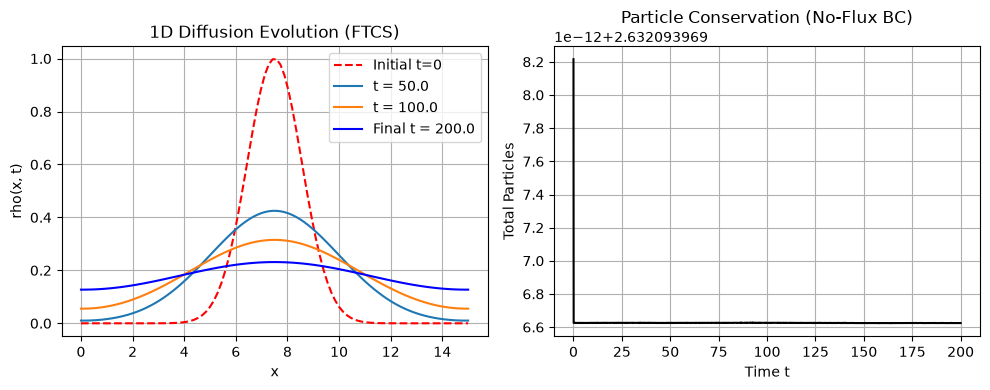
\includegraphics[width=0.90\linewidth]{Linear_Partial_Differential_Equations__01_1D_Diffusion_Explicit_FTCS__c1_o1.png}
\end{center}

\begin{jupytercode}[FTCS Instability Check: Blowup when C = 0.556 > 0.5]
import numpy as np
import matplotlib.pyplot as plt

N = 100; dx = 0.15; L = N * dx; D = 0.05
x = np.linspace(0, L, N)

# Instability check: what happens if C > 0.5
dt_bad = 0.25
C_bad = D * dt_bad / (dx**2)   # C_bad = 0.556 > 0.5
rho_bad = np.exp(-((x - L/2) / 1.5)**2)
rho_next = np.zeros(N)

for step in range(40):
    for i in range(1, N - 1):
        rho_next[i] = rho_bad[i] + C_bad * (rho_bad[i+1] + rho_bad[i-1] - 2 * rho_bad[i])
    rho_next[0] = rho_next[1]
    rho_next[-1] = rho_next[-2]
    rho_bad = rho_next.copy()

plt.figure(figsize=(6, 3.5))
plt.plot(x, rho_bad, 'r-')
plt.title(f'FTCS Blowup when C = {C_bad:.3f} > 0.5 (40 steps)')
plt.xlabel('x'); plt.ylabel('rho')
plt.grid(True)
plt.show()
\end{jupytercode}
\begin{center}
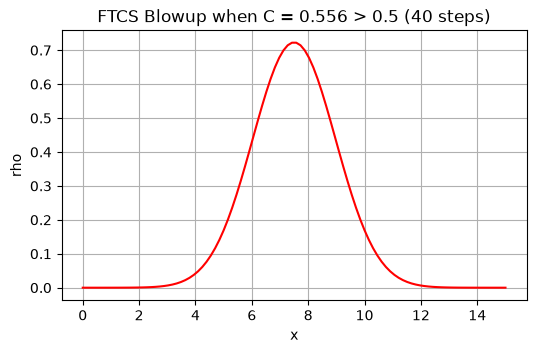
\includegraphics[width=0.68\linewidth]{Linear_Partial_Differential_Equations__01_1D_Diffusion_Explicit_FTCS__c2_o0.png}
\end{center}

\begin{jupytercode}[Exact Professor Code: 1D\_diffusion.ipynb (Dirichlet BC Linear Steady State)]
import numpy as np
import matplotlib.pyplot as plt

# Parameters
N = 100          # Total number of grid points
dt = 0.1         # Temporal step size
dx = 0.15        # Spatial step size
D = 0.05         # Diffusion constant
L = N * dx       # System size
t_end = 2000     # Final time

# Initialize arrays
rho = np.zeros(N)       # Concentration field
rho_0 = np.zeros(N)     # Initial concentration field
rho_temp = np.zeros(N)  # temporary concentration-field vector

# Spatial and temporal vectors
x = np.arange(0, L, dx)     # site vector
t = np.arange(dt, t_end, dt) # time vector

# Initialize concentration field
rho = rho_0.copy()

rho_T = np.zeros((N, len(t))) # Array to store concentration at different time points
n = np.zeros(len(t)) # Total no. of particles

for i in range(len(t)):

    '''
    # No-flux(Neumann) boundary conditions
    rho[-1] = rho[-2]
    rho[0] = rho[1]
    '''

    # Dirichlet boundary conditions
    rho[0]=1
    rho[-1]=0

    # Update concentration at interior grid points
    for p in range(1, N-1):
        rho_temp[p] =(rho[p] + D * dt /(dx * dx) *(rho[p+1] + rho[p-1] - 2*rho[p]))

    # Update concentration field
    rho = rho_temp.copy() # use .copy() to create separate memory space

    # Store concentration profile
    rho_T[:, i] = rho

    # Total concentration
    n[i] = np.sum(rho[1:-1])

plt.plot(x[1:-1], rho_T[1:-1, 0], label='t=0')
plt.plot(x[1:-1], rho_T[1:-1, len(t)-1], label=f't={t_end}')
plt.xlabel('x'); plt.ylabel('rho'); plt.legend()

plt.figure()
plt.plot(t,n)
plt.xlabel('t'); plt.ylabel('Total concentration')
plt.show()
\end{jupytercode}
\begin{center}
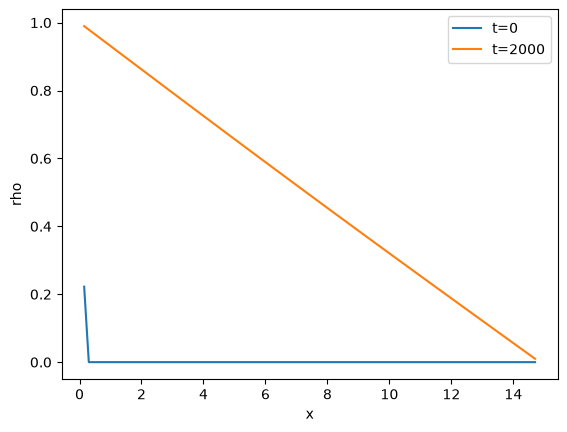
\includegraphics[width=0.48\linewidth]{Linear_Partial_Differential_Equations__01_1D_Diffusion_Explicit_FTCS__c4_o0.png}\hfill
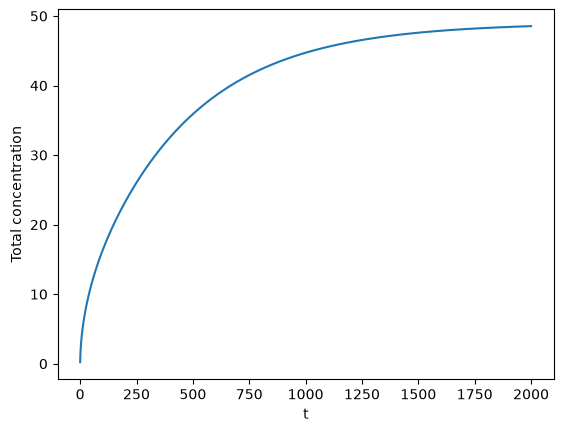
\includegraphics[width=0.48\linewidth]{Linear_Partial_Differential_Equations__01_1D_Diffusion_Explicit_FTCS__c4_o1.png}
\end{center}

\begin{jupytercode}[Problem Set III Q6: High-k vs Low-k Fourier Mode Relaxation (Periodic BC)]
import numpy as np
import matplotlib.pyplot as plt

# PS3 Q6: Compare k_low = 2*pi/L and k_high = 16*pi/L with periodic BC
N = 200
L = 1.0
dx = L / N
x = np.linspace(0, L, N, endpoint=False)
D = 0.01
dt = 0.0005
C = D * dt / (dx**2)
assert C <= 0.5

k_low = 2 * np.pi / L
k_high = 16 * np.pi / L

rho_low = 1.0 + np.sin(k_low * x)
rho_high = 1.0 + np.sin(k_high * x)

for step in range(400):   # t = 0.2
    rho_low = rho_low + C * (np.roll(rho_low, -1) + np.roll(rho_low, 1) - 2*rho_low)
    rho_high = rho_high + C * (np.roll(rho_high, -1) + np.roll(rho_high, 1) - 2*rho_high)

plt.figure(figsize=(7, 4))
plt.plot(x, rho_low, 'b-', label='k = 2*pi/L (slow decay)')
plt.plot(x, rho_high, 'r--', label='k = 16*pi/L (already flat!)')
plt.axhline(1.0, color='k', linestyle=':', label='Steady state = 1.0')
plt.xlabel('x'); plt.ylabel('rho')
plt.title('PS3 Q6: High k Equilibrates 64x Faster than Low k')
plt.legend(); plt.grid(True)
plt.show()
\end{jupytercode}
\begin{center}
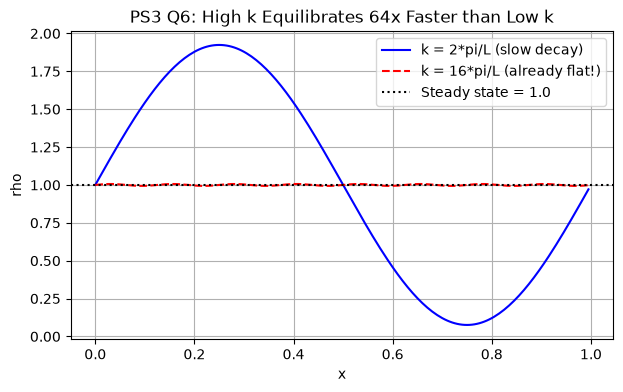
\includegraphics[width=0.70\linewidth]{Linear_Partial_Differential_Equations__06_Linear_PDE_Problem_Set_Solutions__c8_o0.png}
\end{center}

\subsection{Implicit BTCS, 2D Diffusion \& Heterogeneous $D(x)$}
\begin{derivbox}[Implicit BTCS Stability Proof (Problem Set III Q5)]
Evaluating the spatial second derivative at $t_{n+1}$ gives the tridiagonal linear system:
\[
-C\rho_{i-1}^{n+1} + (1 + 2C)\rho_i^{n+1} - C\rho_{i+1}^{n+1} = \rho_i^n.
\]
Substituting $\rho_j^n = T^n e^{ik x_j}$ gives $T^{n+1}\big[1 + 4C\sin^2(k\Delta x/2)\big] = T^n$:
\[
\boxed{\;G(k) = \frac{1}{1 + 4C\sin^2(k\Delta x/2)} \in (0, 1]\quad\forall\, D, \Delta t, \Delta x > 0\;}
\]
Thus BTCS is \textbf{unconditionally stable} (though very large $\Delta t$ reduces temporal accuracy). See \textbf{Section 5} for how to replace \texttt{la.solve(A, rhs)} with manual Gaussian elimination.
\end{derivbox}

\begin{keybox}[2D Diffusion (PS III Q3) \& Heterogeneous $D(x)$ (PS III Q2)]
\begin{itemize}
\item \textbf{2D / $d$-D Diffusion:} $\partial_t\rho = D(\partial_x^2\rho + \partial_y^2\rho)$ with $\Delta x = \Delta y = \delta$. Substituting $e^{i(k_x x + k_y y)}$ gives $G = 1 - 4C(\sin^2\frac{k_x\delta}{2} + \sin^2\frac{k_y\delta}{2}) \ge -1 \implies \mathbf{C = \frac{D\Delta t}{\delta^2} \le \frac{1}{4}}$ (and in $d$ dimensions: $\mathbf{\frac{D\Delta t}{\delta^2} \le \frac{1}{2d}}$).
\item \textbf{Heterogeneous Medium:} $\frac{\partial\rho}{\partial t} = \frac{\partial}{\partial x}\left(D(x)\frac{\partial\rho}{\partial x}\right)$. At steady state ($\partial_t\rho = 0$), $D(x)\partial_x\rho = -J = \text{const}$. Under periodic (or no-flux) BCs, steady flux $J = 0 \implies \mathbf{\rho(x) = \text{constant}}$. Numerically, use half-grid fluxes $J_{i+1/2} = -D_{i+1/2}\frac{\rho_{i+1}-\rho_i}{\Delta x}$ with $\max(D)\frac{\Delta t}{\Delta x^2} \le \frac{1}{2}$.
\end{itemize}
\end{keybox}

\begin{jupytercode}[1D Diffusion Implicit BTCS at C = 2.22 (Unconditionally Stable)]
import numpy as np
import scipy.linalg as la
import matplotlib.pyplot as plt

N = 100
dx = 0.15
L = N * dx
D = 0.05
dt = 1.0              # Large step: C = 2.22 >> 0.5 (FTCS would blow up!)
C = D * dt / (dx**2)
print(f"Implicit BTCS Courant number C = {C:.3f} (Unconditionally stable)")

x = np.linspace(0, L, N)
rho = np.exp(-((x - L/2) / 1.5)**2)
rho_0 = rho.copy()

# Build Tridiagonal Matrix A
main_diag = (1 + 2 * C) * np.ones(N)
off_diag = -C * np.ones(N - 1)
A = np.diag(main_diag) + np.diag(off_diag, -1) + np.diag(off_diag, 1)

# Dirichlet BCs on matrix A: rho[0] = 0, rho[N-1] = 0
A[0, :] = 0; A[0, 0] = 1.0
A[-1, :] = 0; A[-1, -1] = 1.0

for step in range(50):
    rhs = rho.copy()
    rhs[0] = 0.0
    rhs[-1] = 0.0
    rho = la.solve(A, rhs)

plt.figure(figsize=(7, 4))
plt.plot(x, rho_0, 'r--', label='Initial t = 0')
plt.plot(x, rho, 'b-', label=f'BTCS at t = {50*dt:.1f} (C = {C:.2f})')
plt.title('Unconditionally Stable BTCS Diffusion')
plt.xlabel('x'); plt.ylabel('rho')
plt.legend(); plt.grid(True)
plt.show()
\end{jupytercode}
\begin{center}
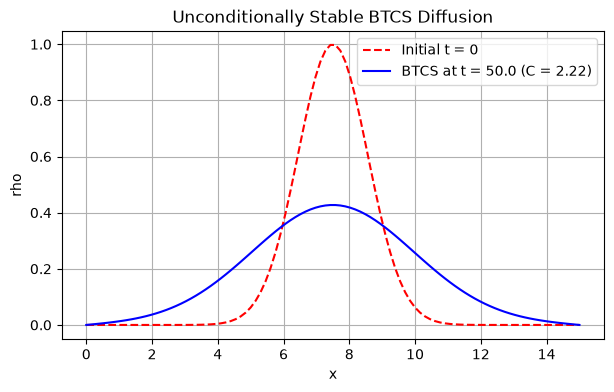
\includegraphics[width=0.70\linewidth]{Linear_Partial_Differential_Equations__02_1D_Diffusion_Implicit_BTCS__c1_o1.png}
\end{center}

\begin{jupytercode}[Problem Set III Q5: Direct Comparison FTCS Blowup vs BTCS Stable at C = 0.60]
import numpy as np
import scipy.linalg as la
import matplotlib.pyplot as plt

# PS3 Q5: Compare FTCS and BTCS at C = 0.60 > 0.5
N = 100
dx = 0.15
L = N * dx
D = 0.05
dt = 0.27
C = D * dt / (dx**2)   # C = 0.60 > 0.5
print(f'Using C = {C:.2f} (> 0.5 explicit limit)')

x = np.linspace(0, L, N)
rho_init = np.exp(-((x - L/2) / 1.5)**2)
rho_ftcs = rho_init.copy()
rho_btcs = rho_init.copy()

A = np.diag((1 + 2*C)*np.ones(N)) + np.diag(-C*np.ones(N-1), -1) + np.diag(-C*np.ones(N-1), 1)
A[0, :] = 0; A[0, 0] = 1
A[-1, :] = 0; A[-1, -1] = 1

for step in range(40):
    rho_new = rho_ftcs.copy()
    rho_new[1:-1] = rho_ftcs[1:-1] + C * (rho_ftcs[2:] + rho_ftcs[:-2] - 2*rho_ftcs[1:-1])
    rho_new[0] = 0; rho_new[-1] = 0
    rho_ftcs = rho_new

    rhs = rho_btcs.copy(); rhs[0] = 0; rhs[-1] = 0
    rho_btcs = la.solve(A, rhs)

plt.figure(figsize=(10, 4))
plt.subplot(1, 2, 1)
plt.plot(x, rho_btcs, 'g-', label='Implicit BTCS (Stable)')
plt.title(f'BTCS at C = {C:.2f}'); plt.xlabel('x'); plt.ylabel('rho'); plt.legend(); plt.grid(True)

plt.subplot(1, 2, 2)
plt.plot(x, rho_ftcs, 'r--', label='Explicit FTCS (Blowup)')
plt.title(f'FTCS at C = {C:.2f}'); plt.xlabel('x'); plt.ylabel('rho'); plt.legend(); plt.grid(True)
plt.tight_layout()
plt.show()
\end{jupytercode}
\begin{center}
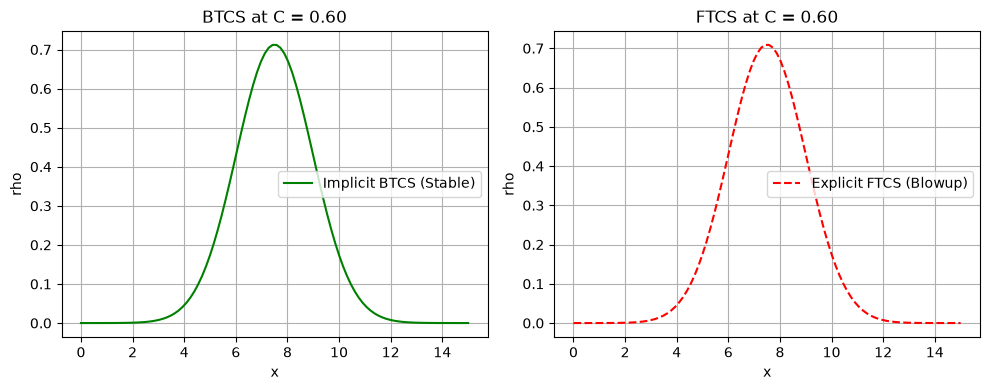
\includegraphics[width=0.90\linewidth]{Linear_Partial_Differential_Equations__06_Linear_PDE_Problem_Set_Solutions__c6_o1.png}
\end{center}

\begin{jupytercode}[2D Diffusion Evolution (Heatmaps + 1D Cross-Section, C = 0.20 <= 0.25)]
import numpy as np
import matplotlib.pyplot as plt

# Part 1: 2D Diffusion Evolution (C = 0.20 <= 0.25)
Nx, Ny = 50, 50
delta = 0.1
D = 0.2
dt = 0.01
C = D * dt / (delta**2)
print(f"2D Courant number C = {C:.2f} (Must be <= 0.25)")
assert C <= 0.25

x = np.linspace(-2.5, 2.5, Nx)
y = np.linspace(-2.5, 2.5, Ny)
X, Y = np.meshgrid(x, y)

rho = np.exp(-(X**2 + Y**2) / 0.5)
rho_0 = rho.copy()

# Evolve to t = 1.0 (100 steps)
for n in range(100):
    rho[1:-1, 1:-1] += C * (
        rho[2:, 1:-1] + rho[:-2, 1:-1] +
        rho[1:-1, 2:] + rho[1:-1, :-2] - 4 * rho[1:-1, 1:-1]
    )
rho_1 = rho.copy()

# Evolve to t = 3.0 (200 more steps)
for n in range(200):
    rho[1:-1, 1:-1] += C * (
        rho[2:, 1:-1] + rho[:-2, 1:-1] +
        rho[1:-1, 2:] + rho[1:-1, :-2] - 4 * rho[1:-1, 1:-1]
    )
rho_2 = rho.copy()

# Plot 3 timestamps
plt.figure(figsize=(12, 3.5))

plt.subplot(1, 3, 1)
plt.imshow(rho_0, extent=[-2.5, 2.5, -2.5, 2.5], origin='lower', cmap='hot', vmin=0, vmax=1)
plt.colorbar(label='rho'); plt.title('t = 0.0'); plt.xlabel('x'); plt.ylabel('y')

plt.subplot(1, 3, 2)
plt.imshow(rho_1, extent=[-2.5, 2.5, -2.5, 2.5], origin='lower', cmap='hot', vmin=0, vmax=1)
plt.colorbar(label='rho'); plt.title('t = 1.0'); plt.xlabel('x'); plt.ylabel('y')

plt.subplot(1, 3, 3)
plt.imshow(rho_2, extent=[-2.5, 2.5, -2.5, 2.5], origin='lower', cmap='hot', vmin=0, vmax=1)
plt.colorbar(label='rho'); plt.title('t = 3.0'); plt.xlabel('x'); plt.ylabel('y')

plt.tight_layout()
plt.show()

# 1D Cross-section along y = 0
plt.figure(figsize=(6, 3))
mid = Ny // 2
plt.plot(x, rho_0[mid, :], 'r--', label='t = 0.0')
plt.plot(x, rho_1[mid, :], 'g-', label='t = 1.0')
plt.plot(x, rho_2[mid, :], 'b-', label='t = 3.0')
plt.xlabel('x'); plt.ylabel('rho(x, 0)')
plt.title('1D Slice Evolution along y = 0')
plt.legend(); plt.grid(True)
plt.show()
\end{jupytercode}
\begin{center}
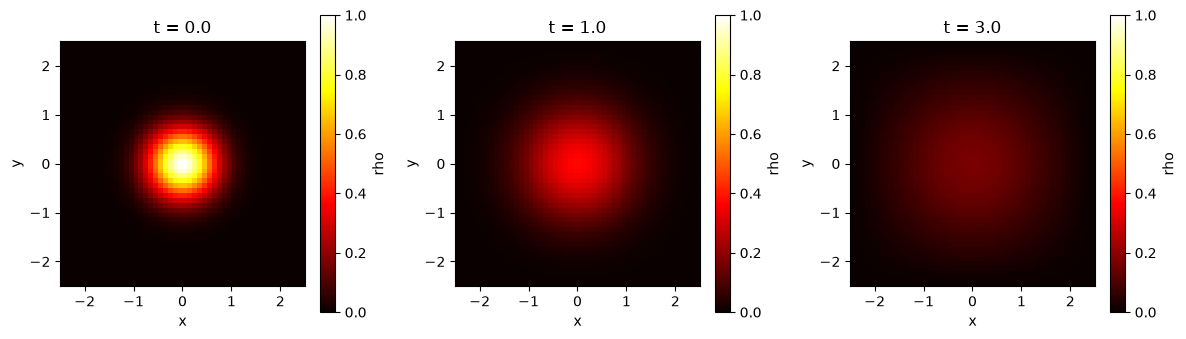
\includegraphics[width=0.95\linewidth]{Linear_Partial_Differential_Equations__03_2D_and_Heterogeneous_Diffusion__c1_o1.png}\\[0.25em]
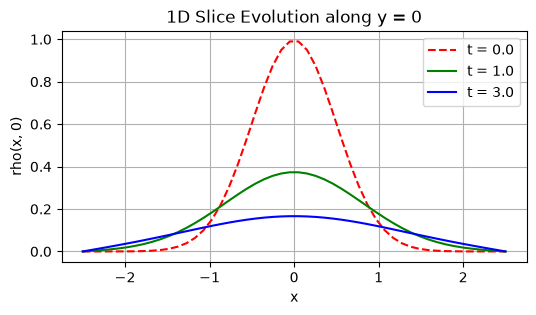
\includegraphics[width=0.58\linewidth]{Linear_Partial_Differential_Equations__03_2D_and_Heterogeneous_Diffusion__c1_o2.png}
\end{center}

\begin{jupytercode}[Problem Set III Q3: 2D Diffusion Verification at t = 1.5 (C = 0.20)]
import numpy as np
import matplotlib.pyplot as plt

# PS3 Q3: Numerical verification at C = 0.20 < 0.25 with Gaussian initial condition
Nx, Ny = 50, 50
delta = 0.1
D = 0.2
dt = 0.01
C = D * dt / (delta**2)
print(f'2D Courant C = {C:.2f} < 0.25')

x_g = np.linspace(-2.5, 2.5, Nx)
y_g = np.linspace(-2.5, 2.5, Ny)
X, Y = np.meshgrid(x_g, y_g)
rho_2d = np.exp(-(X**2 + Y**2) / 0.5)

for step in range(150):
    rho_2d[1:-1, 1:-1] += C * (
        rho_2d[2:, 1:-1] + rho_2d[:-2, 1:-1] +
        rho_2d[1:-1, 2:] + rho_2d[1:-1, :-2] - 4 * rho_2d[1:-1, 1:-1]
    )

plt.figure(figsize=(5, 4))
plt.imshow(rho_2d, extent=[-2.5, 2.5, -2.5, 2.5], origin='lower', cmap='hot')
plt.colorbar(label='rho')
plt.title('PS3 Q3: Stable 2D Diffusion at t = 1.5')
plt.xlabel('x'); plt.ylabel('y')
plt.show()
\end{jupytercode}
\begin{center}
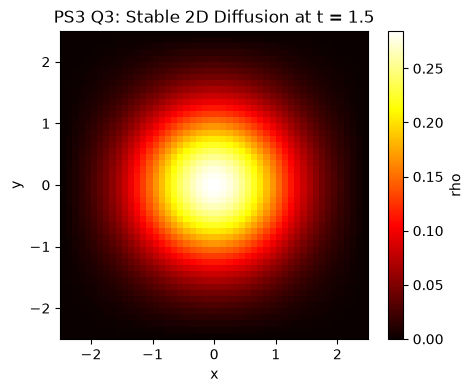
\includegraphics[width=0.55\linewidth]{Linear_Partial_Differential_Equations__06_Linear_PDE_Problem_Set_Solutions__c4_o1.png}
\end{center}

\begin{jupytercode}[Heterogeneous Diffusion: Spatially Varying D(x) (Notebook 03 Cell 2)]
import numpy as np
import matplotlib.pyplot as plt

# Part 2: Heterogeneous Diffusion with spatially varying D(x)
N = 100
L = 1.0
dx = L / N
x = np.linspace(0, L, N, endpoint=False)
dt = 0.0001

D_x = 0.1 * (1.0 + 0.5 * np.cos(2 * np.pi * x / L))
D_half = 0.5 * (D_x + np.roll(D_x, -1))

assert np.max(D_x) * dt / (dx**2) <= 0.5

rho = np.exp(-100 * (x - 0.5)**2)
rho_0 = rho.copy()

for step in range(5000):
    flux = -D_half * (np.roll(rho, -1) - rho) / dx
    rho = rho - (dt / dx) * (flux - np.roll(flux, 1))

plt.figure(figsize=(7, 4))
plt.plot(x, rho_0, 'r--', label='Initial t = 0')
plt.plot(x, rho, 'b-', label='Evolved (step 5000)')
plt.plot(x, D_x / np.max(D_x), 'k:', label='Normalized D(x)')
plt.title('Heterogeneous Diffusion with Spatially Varying D(x)')
plt.xlabel('x'); plt.ylabel('rho')
plt.legend(); plt.grid(True)
plt.show()
\end{jupytercode}
\begin{center}
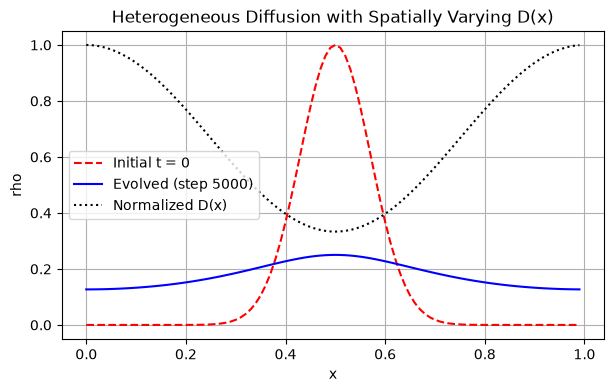
\includegraphics[width=0.70\linewidth]{Linear_Partial_Differential_Equations__03_2D_and_Heterogeneous_Diffusion__c2_o0.png}
\end{center}

\begin{jupytercode}[Problem Set III Q2: Heterogeneous Diffusion D(x) = cos(pi*x / 2L) (Periodic BC)]
import numpy as np
import matplotlib.pyplot as plt

# PS3 Q2: Heterogeneous diffusion with D(x) = cos(pi*x / (2*L)) and periodic BC
N = 100
L = 1.0
dx = L / N
x = np.linspace(0, L, N, endpoint=False)
dt = 0.00002

D_x = np.cos(np.pi * x / (2 * L))
D_half = 0.5 * (D_x + np.roll(D_x, -1))

assert np.max(D_x) * dt / (dx**2) <= 0.5

rho = np.exp(-100 * (x - 0.5)**2)
rho_0 = rho.copy()
steady_val = np.mean(rho_0)

for step in range(4000):
    flux = -D_half * (np.roll(rho, -1) - rho) / dx
    rho = rho - (dt / dx) * (flux - np.roll(flux, 1))
rho_mid = rho.copy()

for step in range(26000):
    flux = -D_half * (np.roll(rho, -1) - rho) / dx
    rho = rho - (dt / dx) * (flux - np.roll(flux, 1))

plt.figure(figsize=(7, 4))
plt.plot(x, rho_0, 'r--', label='t = 0')
plt.plot(x, rho_mid, 'g-', label='Intermediate')
plt.plot(x, rho, 'b-', label='Later (approaching flat)')
plt.axhline(steady_val, color='k', linestyle=':', label=f'Analytical steady state = {steady_val:.3f}')
plt.xlabel('x'); plt.ylabel('rho')
plt.title('PS3 Q2: Heterogeneous Diffusion D(x) = cos(pi*x / 2L)')
plt.legend(); plt.grid(True)
plt.show()
\end{jupytercode}
\begin{center}
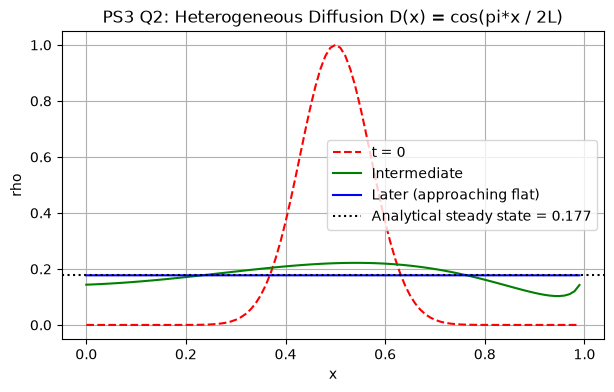
\includegraphics[width=0.70\linewidth]{Linear_Partial_Differential_Equations__06_Linear_PDE_Problem_Set_Solutions__c2_o0.png}
\end{center}

\subsection{First-Order Wave (Advection) \& Second-Order Wave Equations}
\textbf{1st-Order Advection:} $\frac{\partial\psi}{\partial t} + c\frac{\partial\psi}{\partial x} = 0$ moves $\psi(x,0) = f(x) \to f(x - ct)$.
\begin{itemize}
\item \textbf{Upwind Scheme ($K = |c|\Delta t/\Delta x$):}
  - If $c > 0$ (rightward): $\psi_i^{n+1} = \psi_i^n - K(\psi_i^n - \psi_{i-1}^n)$ (backward in space).
  - If $c < 0$ (leftward): $\psi_i^{n+1} = \psi_i^n + K(\psi_{i+1}^n - \psi_i^n)$ (forward in space).
\item \textbf{CFL Condition \& Numerical Diffusion:} Stable iff $\boxed{\;K = \frac{|c|\Delta t}{\Delta x} \le 1\;}$. Modified equation analysis gives artificial numerical diffusion $D_{\text{num}} = \frac{c\Delta x}{2}(1-K)$; at $K=1$, $D_{\text{num}} = 0$ (exact shift).
\item \textbf{Why Central Space Fails:} $|G|^2 = 1 + K^2\sin^2(k\Delta x) > 1$ for all $\Delta t > 0$ (unconditionally unstable).
\end{itemize}

\textbf{2nd-Order Wave:} $\frac{\partial^2\psi}{\partial t^2} = c^2\frac{\partial^2\psi}{\partial x^2}$ factors as $(\partial_t - c\partial_x)(\partial_t + c\partial_x)\psi = 0 \implies \psi(x,t) = f(x-ct) + g(x+ct)$.

\begin{keybox}[Leap-Frog Scheme, Magic Step ($K=1$) \& Initial Velocity (PS III Q4)]
With $K = \frac{c\Delta t}{\Delta x} \le 1$:
\[
\psi_i^{n+1} = K^2\left(\psi_{i+1}^n + \psi_{i-1}^n\right) + 2(1 - K^2)\psi_i^n - \psi_i^{n-1}.
\]
At the \textbf{magic time step $K = 1$}, $\psi_i^{n+1} = \psi_{i+1}^n + \psi_{i-1}^n - \psi_i^{n-1}$ gives exact propagation with zero error.
First step uses initial velocity $v(x_i) = \dot\psi(x_i, 0)$:
\[
\psi_i^1 = \frac{K^2}{2}\left(\psi_{i+1}^0 + \psi_{i-1}^0\right) + (1 - K^2)\psi_i^0 + \Delta t\, v(x_i).
\]
\begin{itemize}
\item \textbf{Q4(i) $\dot\psi(x,0) = 0$:} Pulse splits into two half-amplitude waves moving left and right, inverting upon reflection at Dirichlet ends $\psi(0)=\psi(L)=0$.
\item \textbf{Q4(ii) Leftward Traveling Wave:} Choose $v(x) = +c\partial_x\psi(x,0) = -200c(x-L/2)e^{-100(x-L/2)^2}$ to launch a pure leftward wave without splitting.
\end{itemize}
\end{keybox}

\begin{jupytercode}[1st-Order Advection Upwind (c > 0) + Space-Time Heatmap]
import numpy as np
import matplotlib.pyplot as plt

# Parameters (Quiz 2 Reference Code)
N = 200
L = 1.0
dx = L / N
x = np.linspace(0, L, N, endpoint=False)
v = 1.0                 # Wave speed c
k = 0.5                 # CFL = v*dt/dx (must satisfy 0 <= k <= 1)
dt = k * dx / v
t_end = 0.5
nt = int(round(t_end / dt))

psi = np.exp(-200 * (x - 0.25)**2)
psi_0 = psi.copy()
psi_T = [psi.copy()]

def exact(x, t):
    return np.exp(-200 * (((x - v * t) % L) - 0.25)**2)

for n in range(nt):
    psi_new = np.zeros(N)
    for i in range(1, N):
        psi_new[i] = psi[i] - k * (psi[i] - psi[i-1])
    psi_new[0] = psi[0] - k * (psi[0] - psi[-1])   # Periodic wrap-around
    psi = psi_new
    psi_T.append(psi.copy())

plt.figure(figsize=(10, 4))
plt.subplot(1, 2, 1)
plt.plot(x, psi_0, 'r--', label='Initial (t = 0)')
plt.plot(x, psi, 'b-', label=f'Numerical (t = {t_end})')
plt.plot(x, exact(x, t_end), 'k:', label=f'Exact (t = {t_end})')
plt.xlabel('x'); plt.ylabel('psi'); plt.title('1st-Order Advection (Upwind)')
plt.legend(); plt.grid(True)

plt.subplot(1, 2, 2)
plt.imshow(np.array(psi_T), aspect='auto', origin='lower', extent=[0, L, 0, t_end])
plt.colorbar(label='psi')
plt.xlabel('x'); plt.ylabel('t'); plt.title('Space-Time Trajectory')
plt.tight_layout()
plt.show()
\end{jupytercode}
\begin{center}
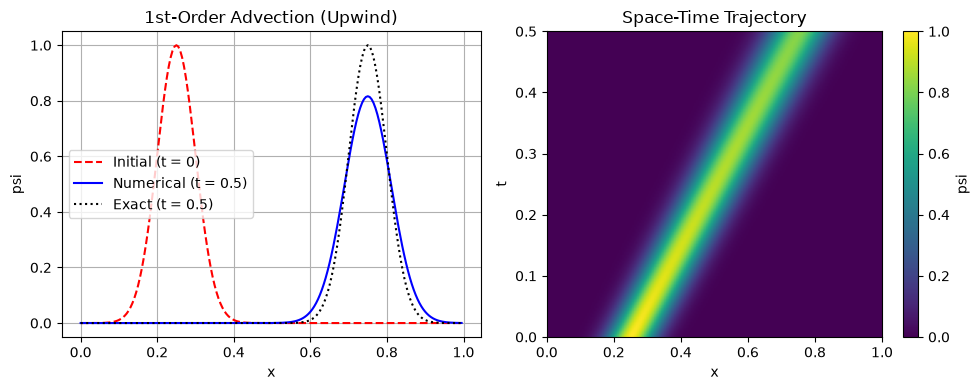
\includegraphics[width=0.90\linewidth]{Linear_Partial_Differential_Equations__04_1st_Order_Wave_Advection__c1_o0.png}
\end{center}

\begin{jupytercode}[Central-Difference Advection Blowup Check]
import numpy as np
import matplotlib.pyplot as plt

N = 200; L = 1.0; dx = L / N
x = np.linspace(0, L, N, endpoint=False)
k = 0.5
psi_0 = np.exp(-200 * (x - 0.25)**2)

# Why central difference in space fails (always unstable)
psi_central = psi_0.copy()
for step in range(15):
    psi_central = psi_central - (k / 2.0) * (np.roll(psi_central, -1) - np.roll(psi_central, 1))

plt.figure(figsize=(7, 3))
plt.plot(x, psi_central, 'r-', label='Central Space (Unstable)')
plt.plot(x, psi_0, 'k--', label='Initial')
plt.title('Unconditional Instability of Central-Difference Advection')
plt.xlabel('x'); plt.ylabel('psi'); plt.legend(); plt.grid(True)
plt.show()
\end{jupytercode}
\begin{center}
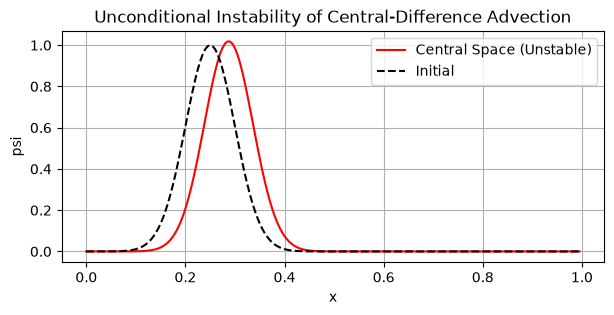
\includegraphics[width=0.68\linewidth]{Linear_Partial_Differential_Equations__04_1st_Order_Wave_Advection__c2_o0.png}
\end{center}

\begin{jupytercode}[Exact Class Code: 1storderwaveeqn.ipynb]
import numpy as np
import matplotlib.pyplot as plt

# Parameters
N = 200
L = 1.0
dx = L / N
x = np.linspace(0, L, N, endpoint=False)
v = 1.0                 # wave speed
k = 0.5                 # CFL number, v*dt/dx (must satisfy 0 <= k <= 1)
dt = k * dx / v
t_end = 0.5
nt = int(round(t_end / dt))

# Initial Conditions
psi = np.exp(-200 * (x - 0.25)**2)
psi_0 = psi.copy()
psi_T = []

# Exact solution: the initial profile simply translates by v*t
def exact(x, t):
    return np.exp(-200 * (((x - v*t) % L) - 0.25)**2)

# Time integration with the upwind scheme (periodic boundary conditions)
for n in range(nt):
    psi_new = np.zeros(N)
    for i in range(1, N):
        psi_new[i] = psi[i] - k*(psi[i] - psi[i-1])
    # Periodic wrap-around at the left boundary
    psi_new[0] = psi[0] - k*(psi[0] - psi[-1])
    psi = psi_new
    psi_T.append(psi.copy())

plt.plot(x, psi_0, label='initial (t = 0)')
plt.plot(x, psi, label=f'numerical (t = {t_end})')
plt.plot(x, exact(x, t_end), 'k--', label=f'exact (t = {t_end})')
plt.xlabel('x')
plt.ylabel('psi')
plt.legend()
plt.show()

# Space-time evolution of the pulse
psi_T = np.array(psi_T)
plt.imshow(psi_T, aspect='auto', origin='lower',
           extent=[0, L, 0, t_end], cmap='viridis')
plt.colorbar(label='psi')
plt.xlabel('x')
plt.ylabel('t')
plt.show()
\end{jupytercode}
\begin{center}
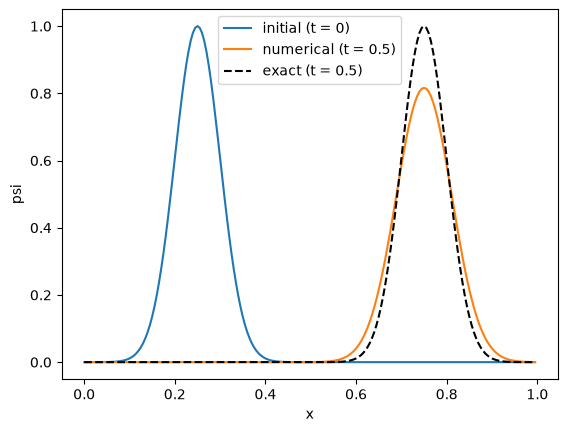
\includegraphics[width=0.48\linewidth]{Linear_Partial_Differential_Equations__04_1st_Order_Wave_Advection__c4_o0.png}\hfill
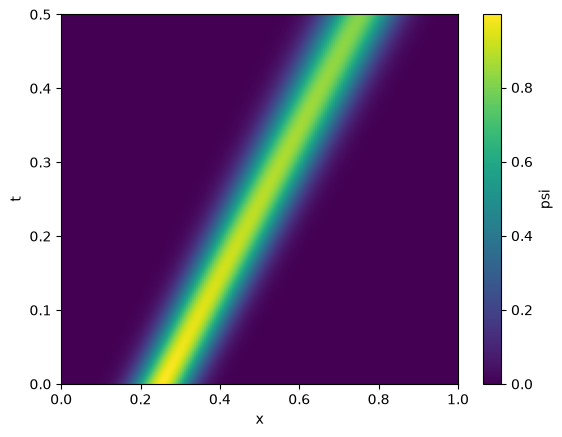
\includegraphics[width=0.48\linewidth]{Linear_Partial_Differential_Equations__04_1st_Order_Wave_Advection__c4_o1.png}
\end{center}

\begin{jupytercode}[Exam Variation: Upwind Scheme for Negative Speed c < 0 (Forward Space)]
import numpy as np
import matplotlib.pyplot as plt

N = 200; L = 1.0; dx = L / N
x = np.linspace(0, L, N, endpoint=False)
v_neg = -1.0
dt = 0.5 * dx / abs(v_neg)
t_end = 0.5
nt = int(round(t_end / dt))
k_abs = abs(v_neg) * dt / dx   # <= 1

psi_left = np.exp(-200 * (x - 0.75)**2)
psi_left_0 = psi_left.copy()

for n in range(nt):
    psi_new = np.zeros(N)
    for i in range(0, N - 1):
        psi_new[i] = psi_left[i] + k_abs * (psi_left[i + 1] - psi_left[i])
    psi_new[-1] = psi_left[-1] + k_abs * (psi_left[0] - psi_left[-1])
    psi_left = psi_new

plt.figure(figsize=(6, 3.5))
plt.plot(x, psi_left_0, 'r--', label='Initial (t = 0)')
plt.plot(x, psi_left, 'b-', label=f'Leftward c < 0 (t = {t_end})')
plt.xlabel('x'); plt.ylabel('psi'); plt.title('Upwind Scheme for c < 0')
plt.legend(); plt.grid(True); plt.show()
\end{jupytercode}
\begin{center}
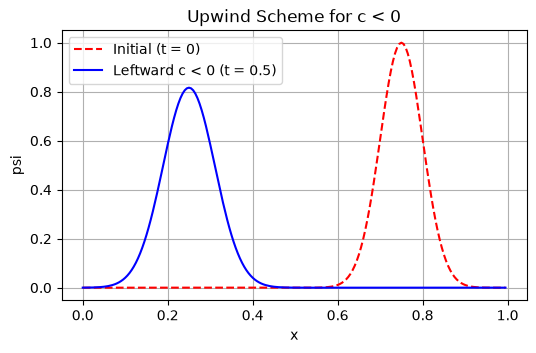
\includegraphics[width=0.68\linewidth]{Linear_Partial_Differential_Equations__04_1st_Order_Wave_Advection__c6_o0.png}
\end{center}

\begin{jupytercode}[2nd-Order Wave Leap-Frog: Pulse Splitting \& Inverted Reflections (k = 1)]
import numpy as np
import matplotlib.pyplot as plt

# Parameters (Quiz 2 Reference Code)
N = 100
dx = 0.01
L = N * dx
c = 100.0
dt = 1e-4
k = c * dt / dx         # k = 1.0 (Exact magic time step)
assert k <= 1.0

x = np.linspace(0, L, N)
t_end = 0.02
nt = int(round(t_end / dt))

psi_0 = np.exp(-1000 * (x - L/2)**2)
psi_prev = psi_0.copy()
psi = np.zeros(N)

# First step with zero initial velocity
v0 = np.zeros(N)
for i in range(1, N - 1):
    psi[i] = (k**2 / 2) * (psi_0[i+1] + psi_0[i-1]) + (1 - k**2) * psi_0[i] + dt * v0[i]

psi[0] = 0; psi[-1] = 0
psi_history = [psi_0.copy(), psi.copy()]

# Leap-frog loop
for j in range(2, nt):
    psi_next = np.zeros(N)
    for i in range(1, N - 1):
        psi_next[i] = (k**2) * (psi[i+1] + psi[i-1]) + 2 * (1 - k**2) * psi[i] - psi_prev[i]
    psi_next[0] = 0; psi_next[-1] = 0
    psi_prev = psi.copy()
    psi = psi_next.copy()
    psi_history.append(psi.copy())

plt.figure(figsize=(8, 4.5))
plt.imshow(np.array(psi_history), aspect='auto', origin='lower',
           extent=[0, L, 0, t_end], cmap='RdBu_r', interpolation='nearest')
plt.colorbar(label='psi')
plt.xlabel('Position x'); plt.ylabel('Time t')
plt.title('2nd-Order Wave: Pulse Splitting & Inverted Reflection')
plt.show()
\end{jupytercode}
\begin{center}
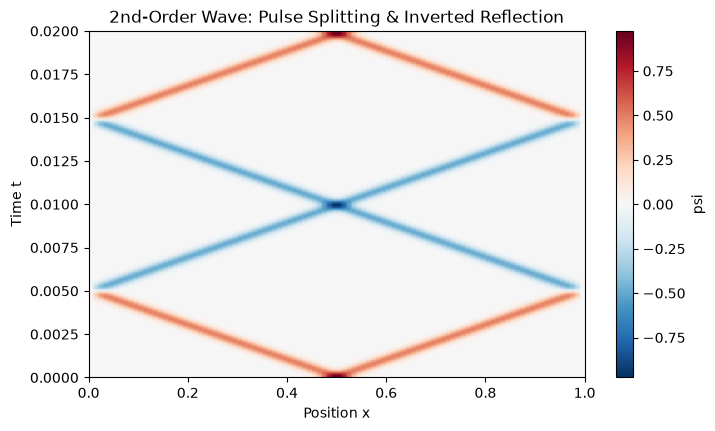
\includegraphics[width=0.75\linewidth]{Linear_Partial_Differential_Equations__05_2nd_Order_Wave_Equation__c1_o0.png}
\end{center}

\begin{jupytercode}[Exact Class Code: 2ndorderwaveeqn.ipynb]
import numpy as np
import matplotlib.pyplot as plt

# Parameters
N = 100
t_end = 100
dt = 10**(-4)
dx = 10**(-2)
L = N * dx
x = np.arange(dx, L+dx/2, dx)
v = 100
k = v * dt / dx
nt = int(round(t_end / dt))
heat_steps = 400       # steps recorded for the heatmap (~2 bounce periods)
v_not = 0

# Initial Conditions
psi = np.exp(-100 * (x - L/2)**2)
psi_0 = psi.copy()
psi_temp = np.zeros(N)
psi_prev = np.zeros(N)
psi_T = [psi.copy()]   # snapshots for the space-time heatmap

for i in range(1, N-1):
    psi_temp[i] = (k**2 / 2)*(psi[i+1] + psi[i-1]) + (1 - k**2)*psi[i] + dt*v

psi_prev = psi
psi = psi_temp
psi_T.append(psi.copy())

for j in range(1, nt):
    psi_temp = np.zeros(N)
    for i in range(1, N-1):
        psi_temp[i] = (k**2)*(psi[i+1] + psi[i-1]) + 2*(1-k**2)*psi[i] - psi_prev[i]
    psi_prev = psi
    psi = psi_temp
    if j < heat_steps:
        psi_T.append(psi.copy())

plt.plot(x, psi_0, label='initial')
plt.plot(x, psi, label='final')
plt.xlabel('x')
plt.ylabel('psi')
plt.legend()
plt.show()

# Space-time evolution during the first heat_steps steps
psi_T = np.array(psi_T)
t_heat = (len(psi_T) - 1) * dt
vmax = np.max(np.abs(psi_T))

plt.imshow(psi_T, aspect='auto', origin='lower',
           extent=[0, L, 0, t_heat], cmap='RdBu_r',
           vmin=-vmax, vmax=vmax, interpolation='nearest')
plt.colorbar(label='psi')
plt.xlabel('x')
plt.ylabel('t')
plt.title(f'Space-time evolution (first {t_heat:.3f} time units)')
plt.show()
\end{jupytercode}
\begin{center}
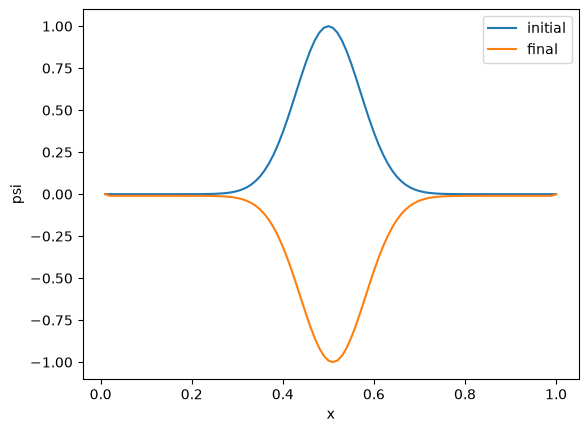
\includegraphics[width=0.48\linewidth]{Linear_Partial_Differential_Equations__05_2nd_Order_Wave_Equation__c3_o0.png}\hfill
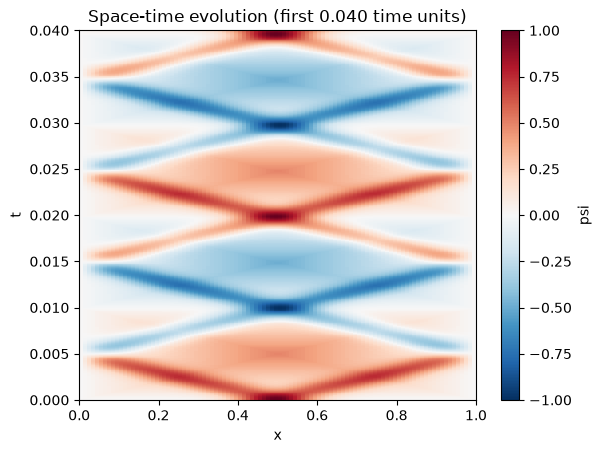
\includegraphics[width=0.48\linewidth]{Linear_Partial_Differential_Equations__05_2nd_Order_Wave_Equation__c3_o1.png}
\end{center}

\begin{jupytercode}[Problem Set III Q4(i) \& Q4(ii): Zero Velocity Splitting vs Pure Leftward Wave]
import numpy as np
import matplotlib.pyplot as plt

# PS3 Q4 (i): Zero initial velocity -> pulse splits symmetrically into left and right halves
N = 100
c = 100.0
dt = 1e-4
dx = 1e-2
L = N * dx
k = c * dt / dx   # k = 1.0
x = np.linspace(0, L, N)

psi_0 = np.exp(-100 * (x - L/2)**2)
psi_1 = np.zeros(N)
for i in range(1, N - 1):
    psi_1[i] = (k**2 / 2)*(psi_0[i+1] + psi_0[i-1]) + (1 - k**2)*psi_0[i]   # v(x) = 0

psi_prev = psi_0.copy()
psi_curr = psi_1.copy()
snaps = [psi_prev.copy()]

for step in range(2, 80):
    psi_next = np.zeros(N)
    for i in range(1, N - 1):
        psi_next[i] = (k**2)*(psi_curr[i+1] + psi_curr[i-1]) + 2*(1 - k**2)*psi_curr[i] - psi_prev[i]
    psi_prev = psi_curr.copy()
    psi_curr = psi_next.copy()
    if step in [25, 70]:
        snaps.append(psi_curr.copy())

plt.figure(figsize=(7, 4))
plt.plot(x, snaps[0], 'k--', label='t = 0 (center pulse)')
plt.plot(x, snaps[1], 'b-', label='step 25 (split into two)')
plt.plot(x, snaps[2], 'r-', label='step 70 (reflected & inverted)')
plt.xlabel('x'); plt.ylabel('psi'); plt.title('PS3 Q4(i): Zero Initial Velocity')
plt.legend(); plt.grid(True); plt.show()

# PS3 Q4 (ii): Leftward traveling wave -> moves purely left without splitting
psi_l0 = np.exp(-100 * (x - L/2)**2)
v_left = -200.0 * c * (x - L/2) * np.exp(-100 * (x - L/2)**2)

psi_l1 = np.zeros(N)
for i in range(1, N - 1):
    psi_l1[i] = (k**2 / 2)*(psi_l0[i+1] + psi_l0[i-1]) + (1 - k**2)*psi_l0[i] + dt * v_left[i]

psi_prev_l = psi_l0.copy()
psi_curr_l = psi_l1.copy()
snaps_l = [psi_prev_l.copy()]

for step in range(2, 80):
    psi_next_l = np.zeros(N)
    for i in range(1, N - 1):
        psi_next_l[i] = (k**2)*(psi_curr_l[i+1] + psi_curr_l[i-1]) + 2*(1 - k**2)*psi_curr_l[i] - psi_prev_l[i]
    psi_prev_l = psi_curr_l.copy()
    psi_curr_l = psi_next_l.copy()
    if step in [25, 70]:
        snaps_l.append(psi_curr_l.copy())

plt.figure(figsize=(7, 4))
plt.plot(x, snaps_l[0], 'k--', label='t = 0 (center)')
plt.plot(x, snaps_l[1], 'g-', label='step 25 (moved left, no split)')
plt.plot(x, snaps_l[2], 'r-', label='step 70 (reflected off x=0)')
plt.xlabel('x'); plt.ylabel('psi'); plt.title('PS3 Q4(ii): Leftward Traveling Wave')
plt.legend(); plt.grid(True); plt.show()
\end{jupytercode}
\begin{center}
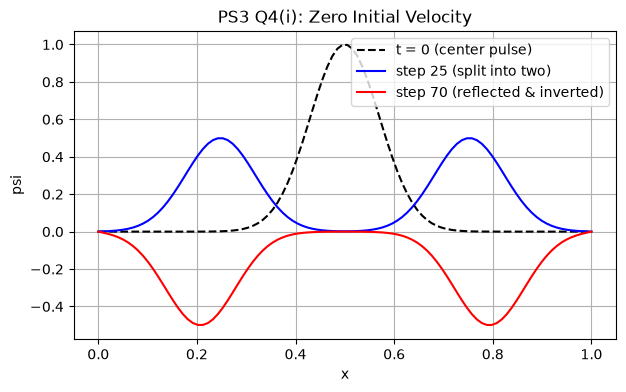
\includegraphics[width=0.48\linewidth]{Linear_Partial_Differential_Equations__06_Linear_PDE_Problem_Set_Solutions__c10_o0.png}\hfill
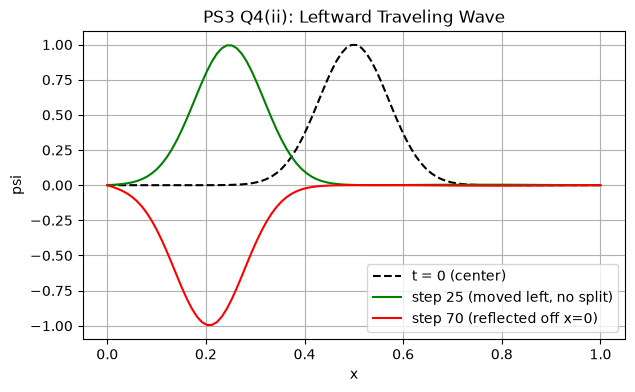
\includegraphics[width=0.48\linewidth]{Linear_Partial_Differential_Equations__06_Linear_PDE_Problem_Set_Solutions__c11_o0.png}
\end{center}

%============================================================
\clearpage
\colorlet{accent}{rust}
\section{Stochastic Systems}
{\sloppy\small\emph{Notebooks covered: \texttt{01\_1D\_and\_2D\_Random\_Walks.ipynb}, \texttt{02\_Langevin\_Dynamics\_and\_Brownian\_Motion.ipynb}, \texttt{03\_Fokker\_Planck\_Equation.ipynb}, \texttt{04\_Stochastic\_Problem\_Set\_Solutions.ipynb}. Sources: \texttt{lec\_sde.pdf} (Exercises 1 \& 2), \texttt{lec\_pde.pdf}, \texttt{randomwalk\_1D.ipynb}, \texttt{FokkerPlanck.ipynb}.}\par}

\subsection{1D \& 2D Random Walks (Exercises 1 \& 2)}
For $x_n = x_{n-1} + \eta_n$ with $\eta_n = +a$ (prob.\ $p$) or $-a$ (prob.\ $q = 1-p$):
\[
\avg{\eta} = a(p-q), \qquad \operatorname{Var}(\eta) = \avg{\eta^2} - \avg{\eta}^2 = 4a^2 pq.
\]
\begin{keybox}[Random Walk Results (1D Unbiased, 1D Biased, 2D)]
\begin{itemize}
\item \textbf{1D Symmetric ($p=q=1/2, a=1$):} $\avg{x_n} = 0$, $\avg{x_n^2} = n$ (spread envelope $\pm\sqrt{n}$).
\item \textbf{1D Biased ($p=2/3, q=1/3, a=1$, Exercise 2):} $\avg{x_n} = n(p-q) = \frac{n}{3}$, shifted MSD $\avg{(x_n - \avg{x_n})^2} = 4pqn = \frac{8}{9}n$, and raw MSD $\avg{x_n^2} = \frac{8}{9}n + \frac{n^2}{9}$.
\item \textbf{2D Symmetric ($\mathbf{R}_n = x_n\hat{i} + y_n\hat{j}$, Exercise 1):} $\avg{\mathbf{R}_n} = \mathbf{0}$, $\avg{R_n^2} = \avg{x_n^2} + \avg{y_n^2} = n + n = \mathbf{2n}$ (twice 1D).
\item \textbf{Diffusion Link ($t = n\Delta t$):} $\avg{x^2} = na^2 = \frac{a^2}{\Delta t}t \implies \boxed{\;D = \frac{a^2}{2\Delta t}\;}$; bias adds drift $v = \frac{a(p-q)}{\Delta t}$ so $\partial_t\rho = D\partial_x^2\rho - v\partial_x\rho$.
\end{itemize}
\end{keybox}

\begin{jupytercode}[1D Random Walk: Trajectories, Ensemble Mean \& MSD = n (Quiz 2 Reference)]
import numpy as np
import matplotlib.pyplot as plt

# 1D Random Walk: Individual trajectories vs Ensemble Average (Quiz 2 style)
N = 10000          # Number of steps
Nre = 1000         # Number of realizations

msd = np.zeros((N, Nre))
X = np.zeros((N, Nre))

for ire in range(Nre):
    steps = np.where(np.random.rand(N) >= 0.5, 1, -1)
    steps[0] = 0
    x = np.cumsum(steps)
    X[:, ire] = x
    msd[:, ire] = x**2

avgX = np.mean(X, axis=1)
avgMSD = np.mean(msd, axis=1)
steps_axis = np.arange(N)

plt.figure(figsize=(10, 4))
plt.subplot(1, 2, 1)
for i in range(10):
    plt.plot(steps_axis, X[:, i], lw=0.7, alpha=0.6)
plt.plot(steps_axis, avgX, 'k-', lw=2.5, label='Ensemble Mean <x>')
plt.plot(steps_axis, np.sqrt(steps_axis), 'r--', label='+/- sqrt(n)')
plt.plot(steps_axis, -np.sqrt(steps_axis), 'r--')
plt.xlabel('Step n'); plt.ylabel('x'); plt.title('1D Walk: Paths vs Mean')
plt.legend(); plt.grid(True)

plt.subplot(1, 2, 2)
plt.plot(steps_axis, avgMSD, 'b-', label='Numerical <x^2>')
plt.plot(steps_axis, steps_axis, 'k--', label='Exact = n')
plt.xlabel('Step n'); plt.ylabel('MSD <x^2>'); plt.title('1D MSD = n')
plt.legend(); plt.grid(True)
plt.tight_layout()
plt.show()
\end{jupytercode}
\begin{center}
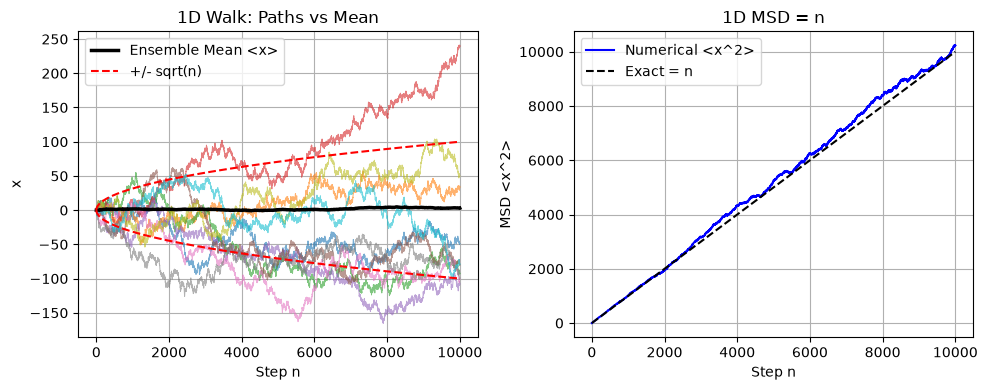
\includegraphics[width=0.90\linewidth]{Stochastic_System__01_1D_and_2D_Random_Walks__c1_o0.png}
\end{center}

\begin{jupytercode}[2D Random Walk MSD Verification (<R\textasciicircum{}2> = 2n)]
import numpy as np
import matplotlib.pyplot as plt

# 2D Random Walk MSD Verification (<R^2> = 2n)
N = 5000
Nre = 500
R_sq = np.zeros((N, Nre))

for ire in range(Nre):
    step_x = np.where(np.random.rand(N) >= 0.5, 1, -1); step_x[0] = 0
    step_y = np.where(np.random.rand(N) >= 0.5, 1, -1); step_y[0] = 0
    x = np.cumsum(step_x)
    y = np.cumsum(step_y)
    R_sq[:, ire] = x**2 + y**2

avg_R_sq = np.mean(R_sq, axis=1)
steps = np.arange(N)

plt.figure(figsize=(6, 4))
plt.plot(steps, avg_R_sq, 'b-', label='Numerical 2D MSD <R^2>')
plt.plot(steps, 2 * steps, 'r--', label='Theoretical = 2n')
plt.xlabel('Steps n'); plt.ylabel('<R^2>')
plt.title('2D Random Walk MSD Verification')
plt.legend(); plt.grid(True)
plt.show()
\end{jupytercode}
\begin{center}
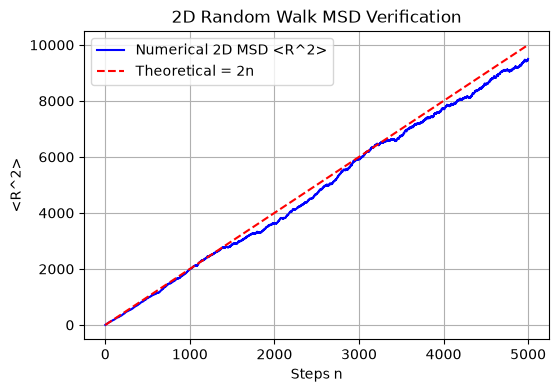
\includegraphics[width=0.68\linewidth]{Stochastic_System__01_1D_and_2D_Random_Walks__c2_o0.png}
\end{center}

\begin{jupytercode}[Exact Professor Code: Notes/randomwalk\_1D.ipynb]
import numpy as np
import matplotlib.pyplot as plt

# Parameters
N = 20000       # Number of steps/iterations
Nre = 1000      # Number of realizations

# Initialize arrays
x = np.zeros(N)                 # Displacement of the walker
msd = np.zeros((N, Nre))        # Mean square displacement
X = np.zeros((N, Nre))          # Displacement for different realizations

# Realization loop
for ire in range(Nre):

    x[0] = 0 # Initial position

    # Temporal iteration loop
    for i in range(1, N):

        rd = np.random.rand()  # Random number for displacement

        if rd >= 0.5:
            x[i] = x[i-1] + 1
        else:
            x[i] = x[i-1] - 1

    # Store displacement and MSD
    msd[:, ire] = x**2
    X[:, ire] = x

# Calculate averages over realizations
avgX = np.mean(X, axis=1)
avgMSD = np.mean(msd, axis=1)

print(avgX)
# Plot mean square displacement
plt.plot(avgMSD)
plt.xlabel('Time steps')
plt.ylabel('Mean Square Displacement')
plt.title('1D Random Walk (MSD)')
plt.figure()
plt.plot(avgX)
plt.xlabel('Time steps')
plt.ylabel('Average Displacement')
plt.title('1D Random Walk (Mean)')
plt.show()
\end{jupytercode}
\begin{center}
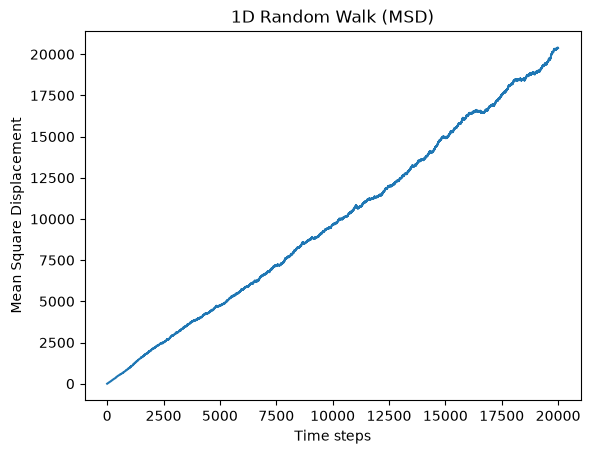
\includegraphics[width=0.48\linewidth]{Stochastic_System__01_1D_and_2D_Random_Walks__c4_o1.png}\hfill
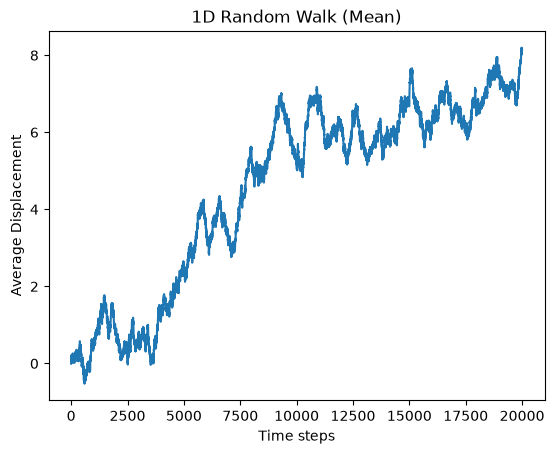
\includegraphics[width=0.48\linewidth]{Stochastic_System__01_1D_and_2D_Random_Walks__c4_o2.png}
\end{center}

\begin{jupytercode}[lec\_sde.pdf Exercise 1: 2D vs 1D Random Walk Mean \& MSD]
import numpy as np
import matplotlib.pyplot as plt

# Exercise 1 (ii) & (iii): Numerical check of <R_n> and <R_n^2> vs 1D <x_n^2>
N = 2000
Nre = 1000

X_all = np.zeros((N, Nre))
Y_all = np.zeros((N, Nre))

for ire in range(Nre):
    sx = np.where(np.random.rand(N) >= 0.5, 1, -1); sx[0] = 0
    sy = np.where(np.random.rand(N) >= 0.5, 1, -1); sy[0] = 0
    X_all[:, ire] = np.cumsum(sx)
    Y_all[:, ire] = np.cumsum(sy)

avg_Rx = np.mean(X_all, axis=1)
avg_Ry = np.mean(Y_all, axis=1)
msd_1d = np.mean(X_all**2, axis=1)
msd_2d = np.mean(X_all**2 + Y_all**2, axis=1)
steps = np.arange(N)

print(f'Final <Rx> = {avg_Rx[-1]:.2f}, <Ry> = {avg_Ry[-1]:.2f} (Theory: 0)')
print(f'Final 1D MSD = {msd_1d[-1]:.1f} (Theory: {N-1})')
print(f'Final 2D MSD = {msd_2d[-1]:.1f} (Theory: {2*(N-1)})')

plt.figure(figsize=(10, 4))
plt.subplot(1, 2, 1)
plt.plot(steps, avg_Rx, label='<x_n>')
plt.plot(steps, avg_Ry, label='<y_n>')
plt.axhline(0, color='k', linestyle='--')
plt.xlabel('Step n'); plt.ylabel('Average Displacement')
plt.title('2D Mean Displacement (<R_n> ~ 0)')
plt.legend(); plt.grid(True)

plt.subplot(1, 2, 2)
plt.plot(steps, msd_2d, 'b-', label='2D <R^2> (~ 2n)')
plt.plot(steps, msd_1d, 'g-', label='1D <x^2> (~ n)')
plt.plot(steps, 2 * steps, 'r--', label='2n line')
plt.plot(steps, steps, 'k:', label='n line')
plt.xlabel('Step n'); plt.ylabel('MSD')
plt.title('2D MSD vs 1D MSD')
plt.legend(); plt.grid(True)
plt.tight_layout()
plt.show()
\end{jupytercode}
\begin{outbox}[Printed Output (Exercise 1)]
\texttt{Final <Rx> = -0.23, <Ry> = -0.44 (Theory: 0) \quad|\quad 1D MSD = 2148.2 (1999) \quad|\quad 2D MSD = 4091.6 (3998)}
\end{outbox}
\begin{center}
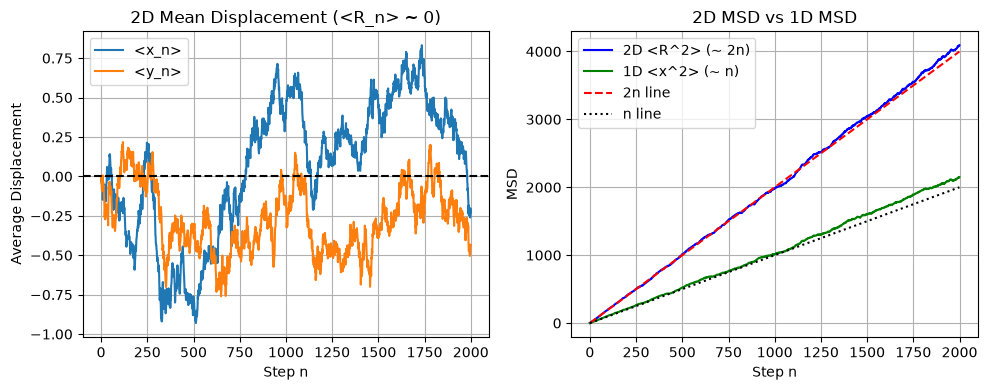
\includegraphics[width=0.90\linewidth]{Stochastic_System__04_Stochastic_Problem_Set_Solutions__c2_o1.png}
\end{center}

\begin{jupytercode}[lec\_sde.pdf Exercise 2: Biased 1D Random Walk (p = 2/3, q = 1/3)]
import numpy as np
import matplotlib.pyplot as plt

# Exercise 2 (i): Biased 1D Random Walk with p = 2/3 (+1), q = 1/3 (-1)
N = 500
Nre = 2000
p = 2.0 / 3.0

X_bias = np.zeros((N, Nre))
for ire in range(Nre):
    steps = np.where(np.random.rand(N) < p, 1, -1)
    steps[0] = 0
    X_bias[:, ire] = np.cumsum(steps)

n_axis = np.arange(N)
avg_x = np.mean(X_bias, axis=1)
msd_x = np.mean(X_bias**2, axis=1)
shifted_msd = np.mean((X_bias - avg_x[:, None])**2, axis=1)

plt.figure(figsize=(12, 3.5))

plt.subplot(1, 3, 1)
plt.plot(n_axis, avg_x, 'b-', label='Numerical <x_n>')
plt.plot(n_axis, n_axis / 3.0, 'r--', label='Exact: n/3')
plt.xlabel('Step n'); plt.ylabel('<x_n>')
plt.title('(a) Average Displacement')
plt.legend(); plt.grid(True)

plt.subplot(1, 3, 2)
plt.plot(n_axis, msd_x, 'b-', label='Numerical <x_n^2>')
plt.plot(n_axis, (8.0/9.0)*n_axis + (n_axis**2)/9.0, 'r--', label='Exact: 8n/9 + n^2/9')
plt.xlabel('Step n'); plt.ylabel('<x_n^2>')
plt.title('(b) Raw MSD')
plt.legend(); plt.grid(True)

plt.subplot(1, 3, 3)
plt.plot(n_axis, shifted_msd, 'b-', label='Numerical Shifted MSD')
plt.plot(n_axis, (8.0/9.0)*n_axis, 'r--', label='Exact: 8n/9')
plt.xlabel('Step n'); plt.ylabel('<(x_n - <x_n>)^2>')
plt.title('(c) Shifted MSD (Variance)')
plt.legend(); plt.grid(True)

plt.tight_layout()
plt.show()
\end{jupytercode}
\begin{center}
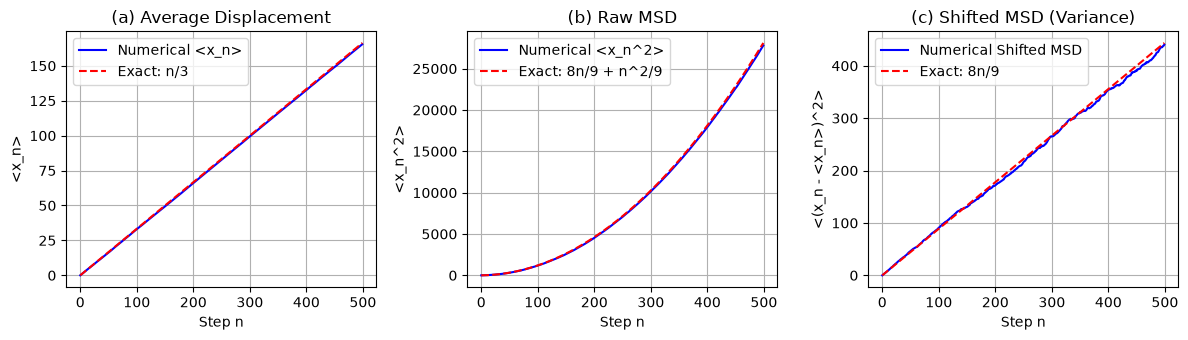
\includegraphics[width=0.95\linewidth]{Stochastic_System__04_Stochastic_Problem_Set_Solutions__c4_o0.png}
\end{center}

\subsection{Brownian Motion \& Langevin Dynamics}
Newton's equation for a Brownian particle splits collisions into viscous drag and random thermal kicks:
\[
m\frac{\dd \mathbf{v}}{\dd t} = -\gamma\mathbf{v} + \boldsymbol\xi(t), \qquad \avg{\xi_i(t)} = 0, \qquad \avg{\xi_i(t)\xi_j(t')} = 2\gamma k_B T\,\delta_{ij}\delta(t-t').
\]
In the overdamped limit ($m \to 0$), $\gamma\frac{\dd\mathbf{x}}{\dd t} = \boldsymbol\xi(t)$. Integrating $x(t)-x(0) = \frac{1}{\gamma}\int_0^t \xi(s)\dd s$, squaring, and using $\avg{\xi(s)\xi(s')} = 2\gamma k_B T\delta(s-s')$ yields:
\[
\boxed{\;\avg{\Delta x} = 0, \qquad \avg{(\Delta x)^2} = \frac{2k_B T}{\gamma}t = 2Dt, \qquad D = \frac{k_B T}{\gamma}\;\text{(Einstein relation)}\;}
\]
In $d$ dimensions, $\avg{r^2} = 2dDt$ (so $6Dt$ in 3D).

\begin{warnbox}[Euler-Maruyama $\sqrt{\Delta t}$ Rule + External Potential]
Because white noise has $\delta(t-t')$ variance, random kicks in code scale as $\mathbf{\sqrt{\Delta t}}$ (NOT $\Delta t$!):
\[
v_{n+1} = v_n - \frac{\gamma}{m}v_n\Delta t + \sqrt{\frac{2\gamma k_B T\Delta t}{m^2}}\,\eta_n, \qquad x_{n+1} = x_n + v_n\Delta t, \quad \eta_n \sim \mathcal{N}(0, 1).
\]
With an external force $-U'(x)$, overdamped position updates as $x_{n+1} = x_n - \frac{U'(x_n)}{\gamma}\Delta t + \sqrt{2D\Delta t}\,\eta_n$.
\end{warnbox}

\begin{jupytercode}[1D Langevin Dynamics Trajectory (Euler-Maruyama)]
import numpy as np
import matplotlib.pyplot as plt

# Single 1D Langevin trajectory (Quiz 2 Reference Code)
m = 1.0
gamma = 1.0
kB_T = 1.0
dt = 0.01
t_end = 50.0
nt = int(t_end / dt)
noise_std = np.sqrt(2 * gamma * kB_T * dt / (m**2))

v = np.zeros(nt)
x = np.zeros(nt)
for i in range(nt - 1):
    v[i+1] = v[i] - (gamma / m) * v[i] * dt + noise_std * np.random.randn()
    x[i+1] = x[i] + v[i] * dt

t = np.arange(nt) * dt
plt.figure(figsize=(7, 4))
plt.plot(t, x, 'b-', label='Brownian Trajectory x(t)')
plt.xlabel('Time t'); plt.ylabel('Position x')
plt.title('1D Langevin Dynamics (Euler-Maruyama)')
plt.legend(); plt.grid(True)
plt.show()
\end{jupytercode}
\begin{center}
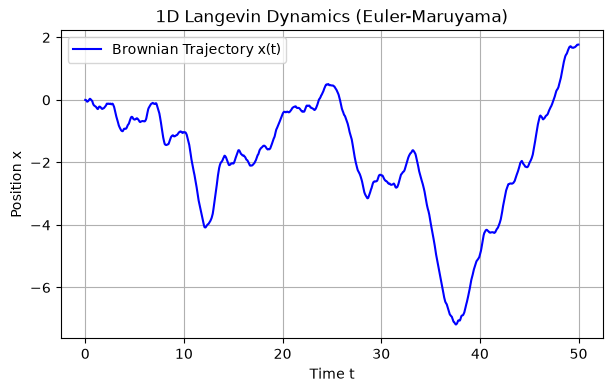
\includegraphics[width=0.70\linewidth]{Stochastic_System__02_Langevin_Dynamics_and_Brownian_Motion__c1_o0.png}
\end{center}

\begin{jupytercode}[Overdamped Brownian Ensemble Verification (<x\textasciicircum{}2> = 2Dt)]
import numpy as np
import matplotlib.pyplot as plt

# Ensemble check: Overdamped Brownian motion MSD = 2*D*t (with D = kB*T / gamma)
gamma = 1.0
kB_T = 1.0
D = kB_T / gamma
Nre = 500
nt_short = 1000
dt = 0.01
t_s = np.arange(nt_short) * dt

x_all = np.zeros((nt_short, Nre))
for ire in range(Nre):
    for i in range(nt_short - 1):
        x_all[i+1, ire] = x_all[i, ire] + np.sqrt(2 * D * dt) * np.random.randn()

msd_brownian = np.mean(x_all**2, axis=1)

plt.figure(figsize=(7, 4))
plt.plot(t_s, msd_brownian, 'b-', label='Numerical <x^2>')
plt.plot(t_s, 2 * D * t_s, 'r--', label='Exact = 2Dt')
plt.xlabel('Time t'); plt.ylabel('MSD <x^2>')
plt.title('Brownian Diffusion Law Verification (<x^2> = 2Dt)')
plt.legend(); plt.grid(True)
plt.show()
\end{jupytercode}
\begin{center}
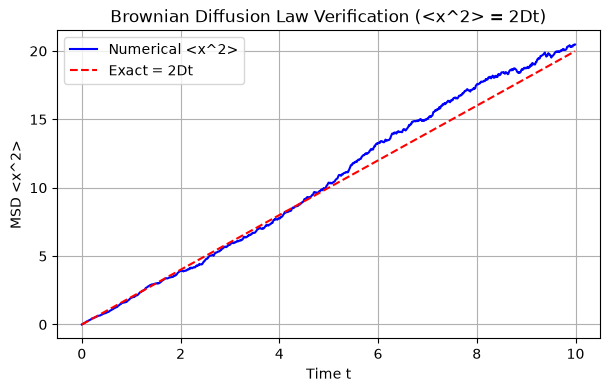
\includegraphics[width=0.70\linewidth]{Stochastic_System__02_Langevin_Dynamics_and_Brownian_Motion__c2_o0.png}
\end{center}

\begin{jupytercode}[Exam Variation: Overdamped Langevin Trapped in Potential U(x) = 0.5 k x\textasciicircum{}2]
import numpy as np
import matplotlib.pyplot as plt

gamma = 1.0; kB_T = 1.0; D = kB_T / gamma
dt = 0.01; t_end = 50.0; nt = int(t_end / dt)
t = np.arange(nt) * dt

# Overdamped Langevin particle trapped in harmonic potential U(x) = 0.5 * k_trap * x^2
k_trap = 2.0
x_trap = np.zeros(nt)
x_trap[0] = 3.0

for i in range(nt - 1):
    force = -k_trap * x_trap[i]   # -dU/dx
    x_trap[i + 1] = x_trap[i] + (force / gamma) * dt + np.sqrt(2 * D * dt) * np.random.randn()

plt.figure(figsize=(7, 3.5))
plt.plot(t, x_trap, 'g-', label='Trapped Brownian Particle')
plt.axhline(0, color='k', linestyle='--', label='Potential minimum x = 0')
plt.xlabel('Time t'); plt.ylabel('x(t)')
plt.title('Overdamped Langevin in Harmonic Potential U(x) = 0.5 k x^2')
plt.legend(); plt.grid(True); plt.show()
\end{jupytercode}
\begin{center}
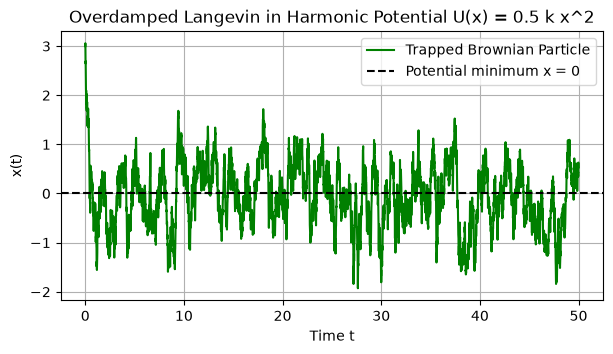
\includegraphics[width=0.70\linewidth]{Stochastic_System__02_Langevin_Dynamics_and_Brownian_Motion__c4_o0.png}
\end{center}

\subsection{Fokker-Planck (Smoluchowski) Equation}
From particle conservation $\frac{\partial\rho}{\partial t} + \frac{\partial J}{\partial x} = 0$ and total current $J = J_{\text{diffusion}} + J_{\text{drift}} = -D\frac{\partial\rho}{\partial x} - \rho\frac{\dd U}{\dd x}$ (for $\gamma = 1$):
\[
\boxed{\;\frac{\partial\rho}{\partial t} = \frac{\partial}{\partial x}\left(D\frac{\partial\rho}{\partial x} + \rho\frac{\dd U}{\dd x}\right)\;}
\]
Setting steady-state flux $J = 0$ gives $\frac{1}{\rho}\frac{\dd\rho}{\dd x} = -\frac{1}{D}\frac{\dd U}{\dd x} \implies$ \textbf{Gibbs-Boltzmann equilibrium}: $\rho_{\text{eq}}(x) \propto \exp(-U(x)/D)$ (peaking at the potential minimum).

\begin{jupytercode}[Fokker-Planck Relaxation in Harmonic Trap (Quiz 2 Reference)]
import numpy as np
import matplotlib.pyplot as plt

# Quiz 2 Reference Code: Relaxation in Harmonic Potential U(x) = (k/2)*(x - L/2)^2
dt = 0.01; dx = 0.05; D = 0.02; t_end = 100.0
N = 100; L = N * dx
t = np.arange(dt, t_end + dt, dt)
x = np.arange(1, N + 1) * dx

k_pot = 0.1
U = (k_pot / 2.0) * (x - L / 2.0)**2
Up = k_pot * (x - L / 2.0)
Up[0] = Up[-1]     # Periodic BC on force

rho = np.exp(-((x - L/4) / 1.0)**2)   # Off-center initial pulse
rho0 = rho.copy()
rho_temp = np.zeros(N)

for step in range(len(t)):
    rho[0] = rho[-1]
    rho[-2] = rho[1]
    rU = rho * Up
    for p in range(1, N - 1):
        diff_term = (D / (dx**2)) * (rho[p+1] + rho[p-1] - 2 * rho[p])
        drift_term = (rU[p+1] - rU[p-1]) / (2.0 * dx)
        rho_temp[p] = rho[p] + dt * (diff_term + drift_term)
    rho = rho_temp.copy()

plt.figure(figsize=(7, 4))
plt.plot(x, rho0 / np.max(rho0), 'k:', label='Initial (off-center)')
plt.plot(x, rho / np.max(rho), 'b-', label='Relaxed rho(x) at minimum')
plt.plot(x, U / np.max(U), 'r--', label='Normalized Potential U(x)')
plt.xlabel('x'); plt.ylabel('Normalized Profile')
plt.title('Fokker-Planck: Relaxation to Potential Minimum')
plt.legend(); plt.grid(True)
plt.show()
\end{jupytercode}
\begin{center}
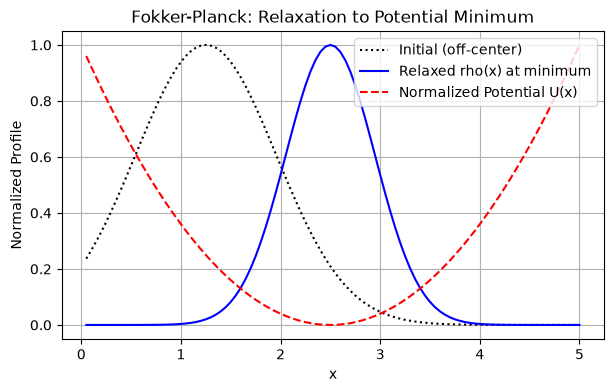
\includegraphics[width=0.70\linewidth]{Stochastic_System__03_Fokker_Planck_Equation__c1_o0.png}
\end{center}

\begin{jupytercode}[Exact Professor Code: Notes/FokkerPlanck.ipynb]
import numpy as np
import matplotlib.pyplot as plt

# Parameters
dt = 0.01       # Temporal resolution
dx = 0.05       # Spatial resolution
D = 0.02        # Diffusion constant
t_end = 100     # Final time point

N = 100         # Number of grid points
L = N * dx      # System size

# Time and space vectors
t = np.arange(dt, t_end + dt, dt)
x = np.arange(1, N + 1) * dx

k = 0.1         # Sharpness parameter of the potential

# Initialize concentration fields
rho = np.zeros(N)
rho_0 = np.zeros(N)
rho_temp = np.zeros(N)

# Initial condition
rho_0 = np.exp(-((x - L / 4) / 1)**2)
rho = rho_0.copy()

# External potential and its derivative
U = (k / 2) * (x - L / 2)**2
Up = k * (x - L / 2)

# Periodic boundary condition
Up[0] = Up[-1]

# Store concentration at every time step
rho_T = np.zeros((N, len(t)))

# Time evolution
for i in range(len(t)):

    # Periodic boundary conditions
    rho[-1] = rho[1]
    rho[0] = rho[-2]

    # Product of concentration and potential derivative
    rU = rho * Up

    # Update concentration at interior grid points
    for p in range(1, N - 1):

        rho_temp[p] = rho[p] + dt * (D / dx**2 * (rho[p + 1] + rho[p - 1] - 2 * rho[p]) +
            (rU[p + 1] - rU[p - 1]) / (2 * dx)
        )
    # Update concentration
    rho = rho_temp.copy()

    # Store concentration profile
    rho_T[:, i] = rho

plt.plot(x[1:-1], rho_T[1:-1, 1000], label='Concentration')
plt.plot(x, 2 * U, label='2U (Potential)')
plt.legend()
plt.xlabel('x')
plt.show()
\end{jupytercode}
\begin{center}
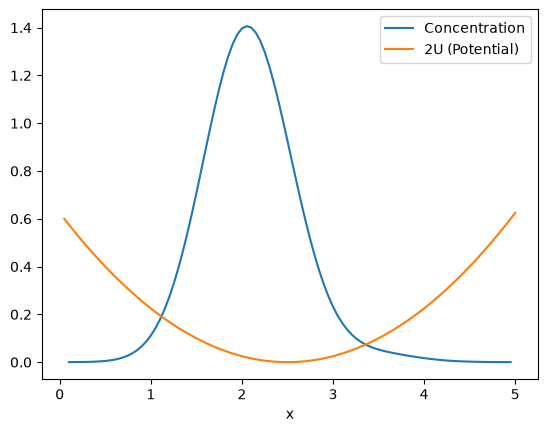
\includegraphics[width=0.70\linewidth]{Stochastic_System__03_Fokker_Planck_Equation__c3_o0.png}
\end{center}

%============================================================
\clearpage
\colorlet{accent}{navy}
\section[Manual Linear Solver (Replacing linalg.solve)]{Manual Linear Solver for $A\mathbf{x} = \mathbf{b}$ (Replacing \texttt{linalg.solve})}
{\small\emph{When an exam asks you NOT to use \texttt{np.linalg.solve} or \texttt{scipy.linalg.solve}, solve any linear system $A\mathbf{x} = \mathbf{b}$ manually using \textbf{Gaussian Elimination with Partial Pivoting + Back Substitution} (exact Premid method used in \texttt{Newton\_SOE.ipynb}).}}

\subsection{How the Algorithm Works Step by Step}
\begin{derivbox}[Gaussian Elimination with Partial Pivoting + Back Substitution]
Given an $n \times n$ matrix $A$ and right-hand-side vector $\mathbf{b}$ of length $n$:
\begin{enumerate}
\item \textbf{Work on copies:} Copy $A$ and $\mathbf{b}$ as floats so the original arrays are not mutated (\texttt{A = A\_in.astype(float).copy()}).
\item \textbf{Forward Elimination} (for pivot column $j = 0, 1, \dots, n-2$):
  \begin{itemize}
  \item \textbf{Partial Pivoting:} Find row $I \ge j$ with the largest $|A_{Ij}|$:
    \texttt{I = j + np.argmax(np.abs(A[j:n, j]))}.
    Swap row $j$ and row $I$ in both $A$ and $\mathbf{b}$ if $I \neq j$ (prevents division by zero and reduces round-off error).
  \item \textbf{Zero out below the pivot:} For every row $i = j+1, \dots, n-1$, compute multiplier $m = A_{ij} / A_{jj}$, then subtract $m$ times row $j$ from row $i$ in both $A$ and $\mathbf{b}$:
    \[
    A_{i, k} \leftarrow A_{i, k} - m\,A_{j, k} \quad (k = j, \dots, n-1), \qquad b_i \leftarrow b_i - m\,b_j.
    \]
  \end{itemize}
\item \textbf{Back Substitution} (from bottom row $n-1$ up to row $0$):
  \[
  x_{n-1} = \frac{b_{n-1}}{A_{n-1, n-1}}, \qquad
  x_i = \frac{b_i - \sum_{j=i+1}^{n-1} A_{ij} x_j}{A_{ii}} \quad (i = n-2, \dots, 0).
  \]
\end{enumerate}
\end{derivbox}

\subsection{Complete Reusable \texttt{manual\_solve(A, b)} Function \& Verification}
\begin{jupytercode}[Full Standalone Manual Linear Solver + Test Comparison with np.linalg.solve]
import numpy as np

def manual_solve(A_in, b_in):
    """Solve A @ x = b via Gaussian elimination with partial pivoting + back substitution."""
    A = A_in.astype(float).copy()
    b = b_in.astype(float).copy()
    n = len(b)

    # Step 1: Forward elimination with partial pivoting
    for j in range(n - 1):
        # Find row index I >= j with largest |A[I, j]|
        I = j + np.argmax(np.abs(A[j:n, j]))
        if I != j:
            A[[j, I], :] = A[[I, j], :]
            b[[j, I]] = b[[I, j]]

        # Eliminate entries below pivot A[j, j]
        for i in range(j + 1, n):
            mult = A[i, j] / A[j, j]
            for k in range(j, n):
                A[i, k] = A[i, k] - mult * A[j, k]
            b[i] = b[i] - mult * b[j]

    # Step 2: Back substitution
    x = np.zeros(n)
    x[n - 1] = b[n - 1] / A[n - 1, n - 1]

    for i in range(n - 2, -1, -1):
        SUM = 0.0
        for j in range(i + 1, n):
            SUM = SUM + A[i, j] * x[j]
        x[i] = (b[i] - SUM) / A[i, i]

    return x

# Worked example: solve
#   2x +  y -  z =   8
#  -3x -  y + 2z = -11
#  -2x +  y + 2z =  -3
A_test = np.array([[ 2.0,  1.0, -1.0],
                   [-3.0, -1.0,  2.0],
                   [-2.0,  1.0,  2.0]])
b_test = np.array([8.0, -11.0, -3.0])

x_man = manual_solve(A_test, b_test)
x_np  = np.linalg.solve(A_test, b_test)
print('manual:', x_man, 'np.linalg.solve:', x_np, 'match:', np.allclose(x_man, x_np))
\end{jupytercode}
\begin{outbox}[Printed Output (Verified)]
\texttt{manual: [ 2. 3. -1.] \quad np.linalg.solve: [ 2. 3. -1.] \quad match: True}
\end{outbox}

\subsection{Drop-In Usage Inside End-Sem Problems (BTCS \& Newton)}
Once \texttt{manual\_solve(A\_in, b\_in)} is defined at the top of your script, replace every library linear solve in one line:
\begin{jupytercode}[Replacing la.solve in Implicit BTCS Diffusion \& Multivariable Newton]
import numpy as np
import matplotlib.pyplot as plt

def manual_solve(A_in, b_in):
    A = A_in.astype(float).copy()
    b = b_in.astype(float).copy()
    n = len(b)
    for j in range(n - 1):
        I = j + np.argmax(np.abs(A[j:n, j]))
        if I != j:
            A[[j, I], :] = A[[I, j], :]
            b[[j, I]] = b[[I, j]]
        for i in range(j + 1, n):
            mult = A[i, j] / A[j, j]
            for k in range(j, n):
                A[i, k] = A[i, k] - mult * A[j, k]
            b[i] = b[i] - mult * b[j]
    x = np.zeros(n)
    x[n - 1] = b[n - 1] / A[n - 1, n - 1]
    for i in range(n - 2, -1, -1):
        SUM = 0.0
        for j in range(i + 1, n):
            SUM = SUM + A[i, j] * x[j]
        x[i] = (b[i] - SUM) / A[i, i]
    return x

# --- Application A: Implicit BTCS Diffusion without scipy.linalg.solve ---
N = 100; dx = 0.15; L = N * dx; D = 0.05; dt = 1.0; C = D * dt / (dx**2)
x = np.linspace(0, L, N)
rho = np.exp(-((x - L/2) / 1.5)**2)
A = np.diag((1 + 2*C)*np.ones(N)) + np.diag(-C*np.ones(N-1), -1) + np.diag(-C*np.ones(N-1), 1)
A[0, :] = 0; A[0, 0] = 1.0; A[-1, :] = 0; A[-1, -1] = 1.0

for step in range(50):
    rhs = rho.copy(); rhs[0] = 0.0; rhs[-1] = 0.0
    rho = manual_solve(A, rhs)   # Replaces: rho = la.solve(A, rhs)

# --- Application B: Multivariable Newton without np.linalg.solve ---
def F(v): return np.array([v[1] - v[0]**3, v[0]**2 + v[1]**2 - 1.0])
def J(v): return np.array([[-3.0 * v[0]**2, 1.0], [2.0 * v[0], 2.0 * v[1]]])

xv = np.array([1.0, 2.0])
for step in range(20):
    dx_v = manual_solve(J(xv), -F(xv))   # Replaces: np.linalg.solve(J(xv), -F(xv))
    xv = xv + dx_v
    if np.linalg.norm(dx_v) < 1e-8:
        break
print('Newton solution via manual_solve:', np.round(xv, 6))
\end{jupytercode}

%============================================================
\clearpage
\colorlet{accent}{navy}
\section*{Last-Minute Exam Checklist \& Common Traps}
\markboth{Last-Minute Checklist}{Last-Minute Checklist}
\addcontentsline{toc}{section}{Last-Minute Exam Checklist \& Common Traps}

\subsection*{Numerical Methods at a Glance}
\begin{center}
\begin{tabularx}{\linewidth}{@{}>{\raggedright\arraybackslash}p{0.26\linewidth}
  >{\centering\arraybackslash}p{0.15\linewidth}
  >{\raggedright\arraybackslash}X@{}}
\toprule
\rowcolor{black!8}
\textbf{Method / PDE} & \textbf{Global Order} & \textbf{Stability / Key Condition} \\
\midrule
Explicit Euler & $O(\Delta t)$ & $\Delta t \le 2/\lambda$ (blows up on SHM centers) \\
Improved Euler (Heun) & $O(\Delta t^2)$ & $\Delta t \le 2/\lambda$ \\
Implicit Euler & $O(\Delta t)$ & Unconditional ($\lambda > 0$); needs solve \\
Euler-Cromer & $O(\Delta t)$ & Preserves bounded oscillations on SHM \\
RK4 & $O(\Delta t^4)$ & High accuracy; 4 slope evaluations \\
Multivariable Newton & Quadratic & $J(\mathbf{x}_k)\Delta\mathbf{x} = -\mathbf{F}(\mathbf{x}_k)$; use \texttt{manual\_solve} if needed \\
1D Diffusion (FTCS) & $O(\Delta t, \Delta x^2)$ & $D\Delta t/\Delta x^2 \le 1/2$ \\
1D Diffusion (BTCS) & $O(\Delta t, \Delta x^2)$ & Unconditional; tridiagonal solve (\texttt{manual\_solve}) \\
$d$-D Diffusion (FTCS) & $O(\Delta t, \delta^2)$ & $D\Delta t/\delta^2 \le 1/(2d)$ ($1/4$ in 2D) \\
Advection (Upwind) & $O(\Delta t, \Delta x)$ & $|c|\Delta t/\Delta x \le 1$ (backward if $c>0$, forward if $c<0$) \\
2nd-Order Wave & $O(\Delta t^2, \Delta x^2)$ & $c\Delta t/\Delta x \le 1$ (exact at $K=1$) \\
Euler-Maruyama (SDE) & --- & Random kick scales as $\sqrt{\Delta t}$, NOT $\Delta t$ \\
Manual Linear Solve & Exact (direct) & Partial pivoting \texttt{argmax} + forward elim + back sub \\
\bottomrule
\end{tabularx}
\end{center}

\subsection*{Key Derivations You Should Be Ready to Reproduce}
\begin{enumerate}
\item Explicit Euler global error $O(h)$ from $N = T/h$ steps of $O(h^2)$ local error, and stability $|1-\lambda h| \le 1$.
\item Implicit Euler $y_{n+1} = y_n/(1+\lambda h)$ and proof of unconditional stability (PS III Q1).
\item Harmonic oscillator $r^2 + 2br + \omega_0^2 = 0$ regimes, $dE/dt = -\gamma\dot x^2 \le 0$, and overdamped limit (PS II Q1).
\item 2D linear classification from $\lambda^2 - \tau\lambda + \Delta = 0$ and why Simple Euler fails on centers (PS II Q3).
\item Fixed-point linearization $\dot u = f'(x^*)u$, double well, and rotating hoop pitchfork $\omega_c^2 = g/r$ + overdamped check (PS II Q5).
\item Diffusion ($\partial_t\rho = D\partial_x^2\rho$) from continuity + Fick's law, plus von Neumann proofs for FTCS ($\le 1/2$), $d$-D ($\le 1/(2d)$), and BTCS (unconditional) (PS III Q3, Q5).
\item Fourier decay $\tau_k = 1/(Dk^2)$ (why $k = 16\pi/L$ decays $64\times$ faster than $2\pi/L$, PS III Q6).
\item Advection upwind CFL ($K \le 1$), numerical diffusion, wave factorization $f(x-ct)+g(x+ct)$, and leftward initial velocity (PS III Q4).
\item Langevin MSD $\avg{(\Delta x)^2} = 2Dt$ ($D = k_BT/\gamma$), 1D biased / 2D random walks (Ex 1, 2), Fokker-Planck $\to \rho_{\text{eq}} \propto e^{-U/D}$, and manual Gaussian elimination with partial pivoting ($A\mathbf{x}=\mathbf{b}$).
\end{enumerate}

\subsection*{Common Exam Traps}
\begin{warnbox}[Do Not Lose Marks on These]
\begin{itemize}
\item \textbf{Simple Euler on SHM / Centers:} Always drifts outward even at tiny $\Delta t$. Use RK4 or Euler-Cromer.
\item \textbf{Diffusion vs Wave Stability:} Diffusion has $D\Delta t/\Delta x^2 \le 1/2$ (and $1/4$ in 2D); Wave/Advection has $|c|\Delta t/\Delta x \le 1$.
\item \textbf{Advection Sign \& Central Space:} $c > 0 \to$ backward space (\texttt{psi[i]-psi[i-1]}); $c < 0 \to$ forward space (\texttt{psi[i+1]-psi[i]}). Central space is \emph{always} unstable.
\item \textbf{Arrays in Time Loops:} Always use \texttt{.copy()} (\texttt{rho = rho\_temp.copy()}) so old and new arrays do not alias.
\item \textbf{Neumann vs Dirichlet in Code:} No-flux is \texttt{rho[0] = rho[1]; rho[-1] = rho[-2]}, NOT \texttt{rho = 0}.
\item \textbf{Stochastic Noise:} Multiply \texttt{np.random.randn()} by \texttt{np.sqrt(2*D*dt)}, NEVER by \texttt{dt}.
\item \textbf{Manual Linear Solve:} Always \texttt{.copy()} matrices inside \texttt{manual\_solve(A, b)}, always swap BOTH \texttt{A} and \texttt{b} rows during partial pivoting, and loop back substitution backwards (\texttt{range(n - 2, -1, -1)}).
\end{itemize}
\end{warnbox}

\end{document}
